\documentclass{article}
\begin{document}

\begin{center}\vspace*{3mm}{\large\color{blue} MXB362}\par\vspace{8mm}
{\Huge\bfseries\color{navy} Computer Lab Portfolio}\par
{\Large\color{blue} Problem Solving Task 2 -- Weeks 8 to 11}\par\vspace{10mm}
\begin{tabular}{|p{42mm}|p{105mm}|}\hline
\textbf{Student}&Owen Ferguson\\[3mm]\hline
\textbf{Student number}&n11595744\\[3mm]\hline\end{tabular}
\end{center}\vspace{6mm}
{\LARGE\bfseries\color{navy} Portfolio contents}\par
{\large\bfseries\color{blue} Week 8 -- Volume Visualisation 2}\par
Task 1: Greyscale stag beetle volume rendering (R)\\
Task 2: Coloured stag beetle isosurface (MATLAB)\\
Additional output: Rotating isosurface animation\par
{\large\bfseries\color{blue} Week 9 -- Visualising Uncertainty}\par
Task 1: Larval dispersal uncertainty animation (MATLAB)\\
Task 2: Three forms of fishery uncertainty (R)\par
{\large\bfseries\color{blue} Week 10 -- Vector Visualisation}\par
Task 1: Direct vector field (quiver plot)\\
Task 2: Poor and improved streamlines\\
Task 3: Line integral convolution, including optional extensions\par
{\large\bfseries\color{blue} Week 11 -- Visualising High Dimensional Data}\par
Task 1: Iris scatter plot matrix\\
Task 2: Principal component projection\\
Task 3: LDA projection vector and Fisher criterion\\
Task 4: Visualising species separation
\clearpage\section*{Week 8 -- Volume Visualisation 2}
Task 1: Produce a greyscale visualisation of the internal and external structure of the stag beetle, viewed from below.

{\large\bfseries\color{blue} Task 1 -- R volume renderer}\par{\small Source: \texttt{submission/code/week8\_volume.R (run from week8)}}\par
\begin{verbatim}
# Run from 3.2/week8. Additive projection along z.
fid <- file('stag_beetle_832x832x494_uint16.raw', 'rb')
beetle_data <- readBin(fid, 'integer', n = 832*832*494, size = 2, signed = FALSE)
close(fid)
beetle_data <- array(beetle_data, dim = c(832, 832, 494))

I <- matrix(1,
            nrow = dim(beetle_data)[1],
            ncol = dim(beetle_data)[2]
)
for (x in 1:dim(beetle_data)[1]) {
  for (y in 1:dim(beetle_data)[2]) {
    I[x,y] <- sum(beetle_data[x, y, ])
  }
}

rotated_I <- t(apply(I, 2, rev))

image(rotated_I, col = gray.colors(256), asp = 1, axes = FALSE, xlab = "", ylab = "")
\end{verbatim}

The renderer sums voxel intensities along the third dimension, implementing additive blending along parallel viewing rays. The resulting greyscale projection shows overlapping internal and external structures. The matrix is rotated before display.
\clearpage\section*{Task 1 -- Greyscale volume projection}
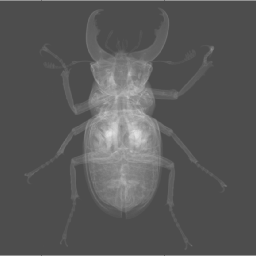
\includegraphics[width=160mm]{figures/beetle_greyscale.png}
\par Saved R output: greyscale additive projection of the stag beetle.

\clearpage\section*{Week 8 -- Coloured isosurface}
Task 2: Render a coloured isosurface with a suitable threshold and viewing angle. The selected isovalue is 400; the volume is subsampled every third voxel and reversed along the third axis.

{\large\bfseries\color{blue} Task 2 -- MATLAB isosurface}\par{\small Source: \texttt{week8/practical8.m}}\par
\begin{verbatim}
fid = fopen('stag_beetle_832x832x494_uint16.raw','r');

data = fread(fid, 832*832*494, 'uint16');

fclose(fid);

D = reshape(data, [832, 832, 494]);
D = D(1:3:end, 1:3:end, end: -3:1);

surface = isosurface(D, 400);

p = patch(surface, 'FaceColor', 'red', 'EdgeColor', 'none');

lighting gouraud
axis equal vis3d off
set(gcf,'color','w')

for t = 1:720
    view([-75+t,19])
    pause(0.025)

    if t == 1 || t == 181
        camlight
    end
end
\end{verbatim}

\clearpage\section*{Task 2 -- Stag beetle isosurface}
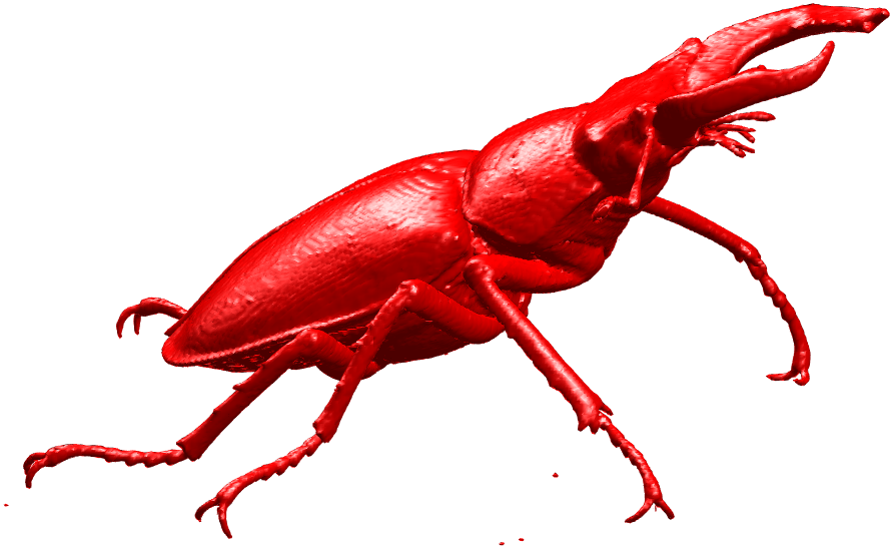
\includegraphics[width=160mm]{../week8/prac8Stag.png}
\par Saved MATLAB output with a red surface and Gouraud lighting; an oblique view reveals the head, mandibles, legs and body.

\clearpage\section*{Week 8 -- Additional animation}
Animation file: \texttt{week8/stag\_beetle\_rotation.mp4}.\par The animation rotates the isosurface through 720 views at 40 frames per second with a headlight that follows the camera. The still image on the preceding page represents the same isosurface task.

{\large\bfseries\color{blue} Rotating isosurface -- MATLAB}\par{\small Source: \texttt{week8/practical8vid.m}}\par
\begin{verbatim}
fid = fopen('stag_beetle_832x832x494_uint16.raw','r');

data = fread(fid, 832*832*494, 'uint16');

fclose(fid);

D = reshape(data, [832, 832, 494]);
D = D(1:3:end, 1:3:end, end:-3:1);

surface = isosurface(D, 400);

p = patch(surface, 'FaceColor', 'red', 'EdgeColor', 'none');

lighting gouraud
axis equal vis3d off
set(gcf,'color','w')

hLight = camlight('headlight');

videoFile = fullfile(fileparts(mfilename('fullpath')), ...
    'stag_beetle_rotation.mp4');

vid = VideoWriter(videoFile, 'MPEG-4');
vid.FrameRate = 40;
vid.Quality = 100;

open(vid);

for t = 1:720
    view([-75+t, 19])

    camlight(hLight, 'headlight')

    drawnow

    frame = getframe(gcf);
    writeVideo(vid, frame);
end

close(vid);

disp(['Video saved to: ' videoFile])
\end{verbatim}

\clearpage\section*{Week 9 -- Visualising Uncertainty}
Task 1: Animate the uncertainty surrounding a larval cloud over time. Green points show individual larval positions and the red convex hull outlines their spatial extent.

{\large\bfseries\color{blue} Task 1 -- MATLAB larval animation}\par{\small Source: \texttt{week9/P9Task1.m}}\par
Animation file: \texttt{week9/LarvalDispersal.gif}. The following page shows four representative frames; the full temporal output is in the GIF.
\begingroup\begin{verbatim}
clear all

figure(1), clf, hold on, box on

load AustOutline_MXB362.mat
pt = patch(Outline(:,1),Outline(:,2),[0.8 0.8 0.8]);
set (pt,'facecolor',[1 0.9 0.65])

load ReefOutline_MXB362.mat
plot(ReefRaw(:,1),ReefRaw(:,2),'b')

xlim([148.5 155]); XL = xlim;
ylim([-25.5 -19.5]); YL = ylim;
set(gca,'color',[0.94 1 1])

load LarvalReleases_MXB362.mat

gifname = 'LarvalDispersal.gif';

nSteps = size(ER_traj_x,1);

for t = 1:nSteps

    x = ER_traj_x(t,:);
    y = ER_traj_y(t,:);

    valid = ~isnan(x) & ~isnan(y);
    x = x(valid);
    y = y(valid);

    P = plot(x,y,'.','markersize',4,'color',[0 0.5 0]);

    if length(x) >= 3
        K = convhull(x,y);
        H = plot(x(K),y(K),'r','linewidth',1.5);
    end

    title(['Larval dispersal - timestep ', num2str(t)])

    drawnow

    frame = getframe(gcf);
    im = frame2im(frame);
    [imind,cm] = rgb2ind(im,256);

    if t == 1
        imwrite(imind,cm,gifname,'gif', ...
            'Loopcount',inf,'DelayTime',0.05);
    else
        imwrite(imind,cm,gifname,'gif', ...
            'WriteMode','append','DelayTime',0.05);
    end

    delete(P)

    if exist('H','var')
        delete(H)
        clear H
    end
end
\end{verbatim}
\endgroup

\clearpage{\Large\bfseries\color{navy} Task 1 -- Larval dispersal animation}\par\begin{center}
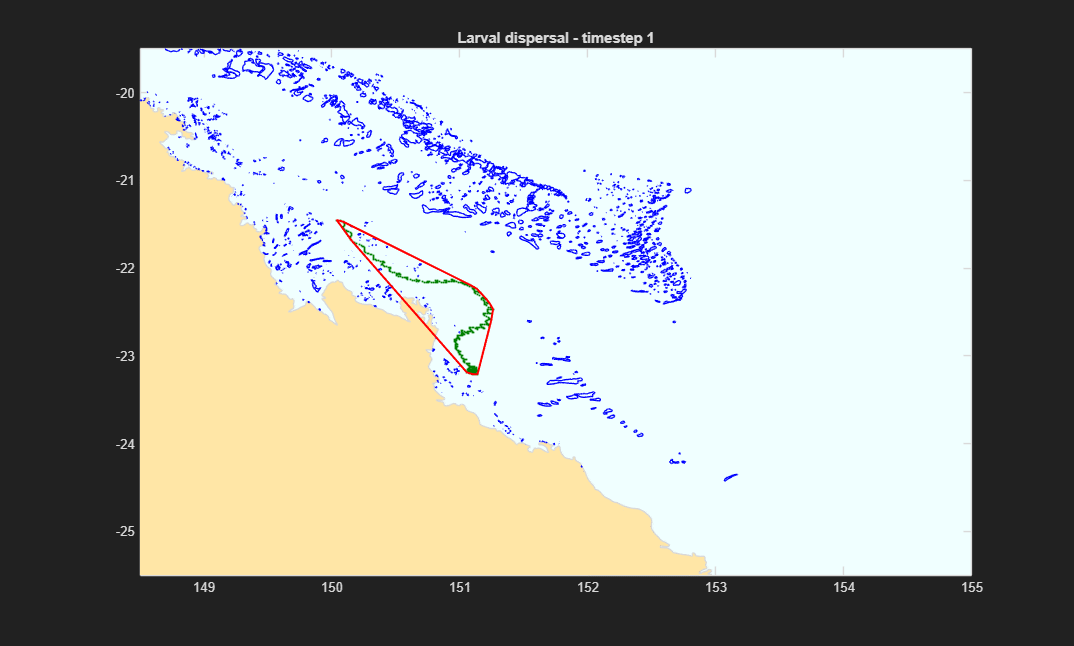
\includegraphics[width=75mm]{figures/larvae_0.png}
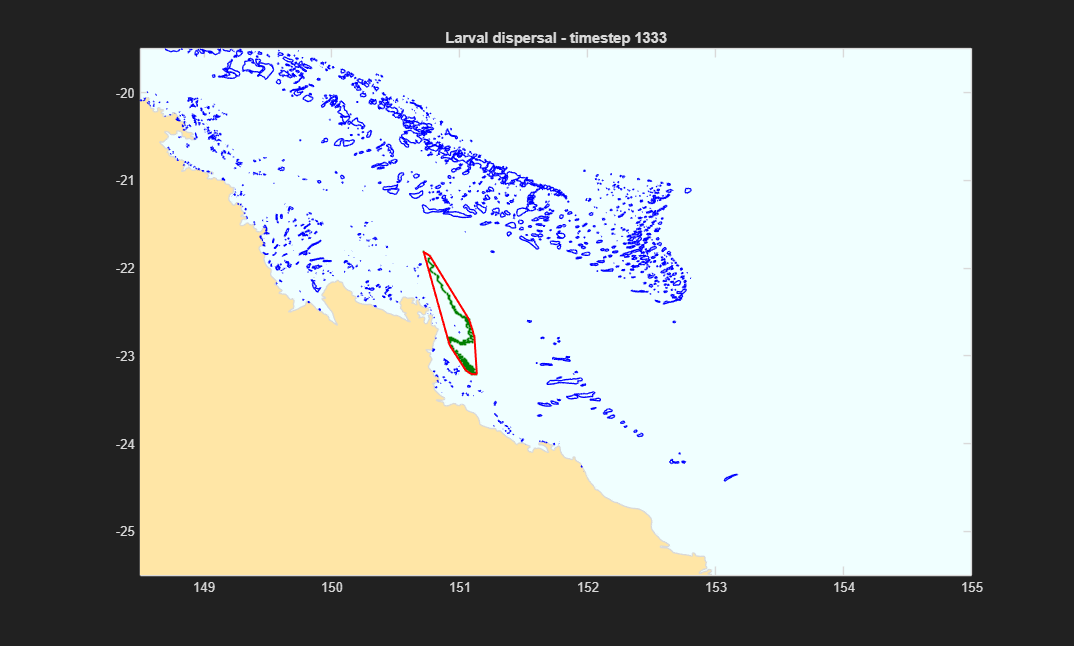
\includegraphics[width=75mm]{figures/larvae_1.png}\par\vspace{4mm}
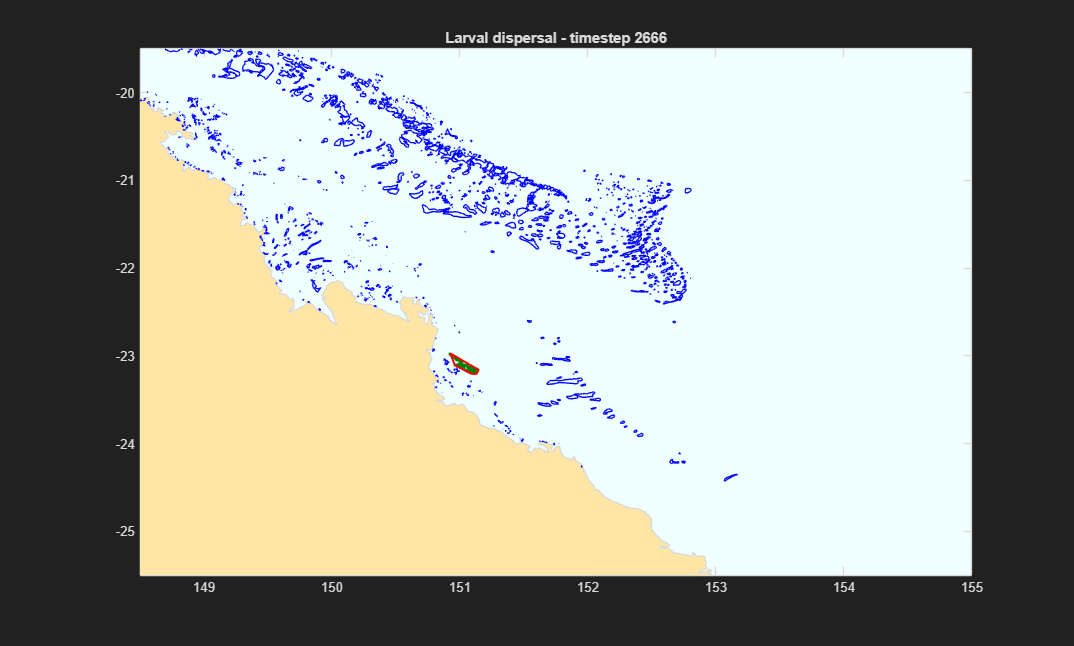
\includegraphics[width=75mm]{figures/larvae_2.png}
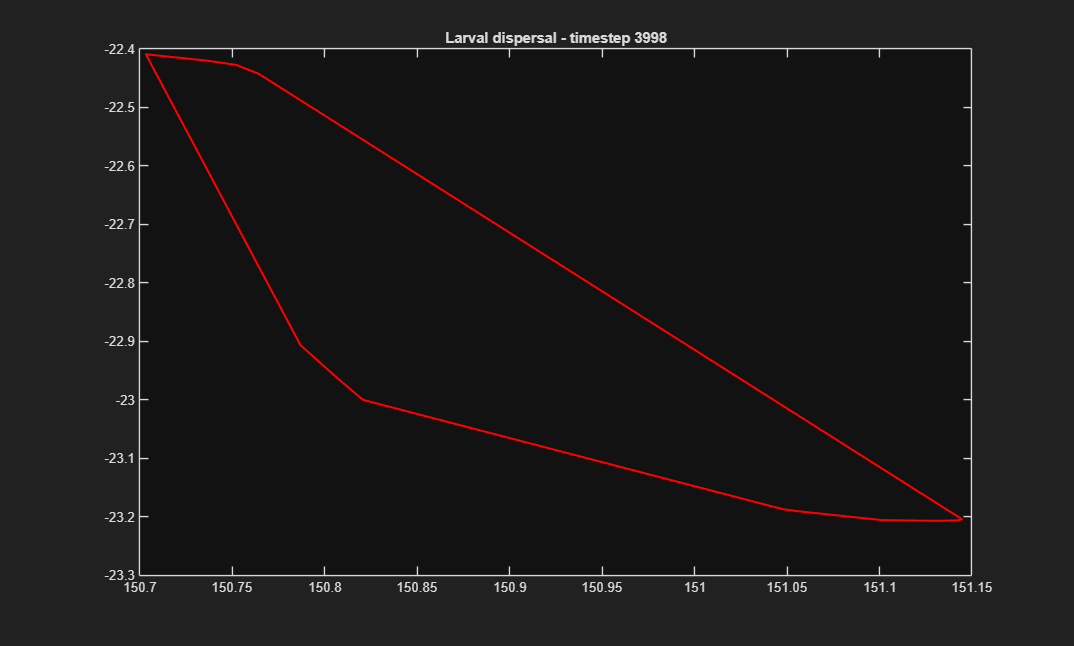
\includegraphics[width=75mm]{figures/larvae_3.png}\par\vspace{4mm}
\end{center}Frames sampled at the beginning, approximately one-third and two-thirds through, and the end of the animation.
\clearpage\section*{Week 9 -- Fishery uncertainty}
Task 2: Show demographic, structural / parametric and scenario uncertainty in a labelled TIFF with legends. The stochastic simulation uses 2,500 replicates over 50 time steps; its shaded interval spans the 2.5th to 97.5th percentiles.

{\large\bfseries\color{blue} Task 2 -- R fishery simulations}\par{\small Source: \texttt{week9/P9Task2.R}}\par
\begin{verbatim}
r <- 0.25
h <- 0.1
st <- 0.25
K <- 1
TMax <- 50
NumReps <- 2500

simulate_population <- function(z, h, stochastic = TRUE) {
  
  N <- matrix(0.5, nrow = NumReps, ncol = TMax)
  
  for (i in 1:NumReps) {
    for (t in 1:(TMax - 1)) {
      
      if (stochastic) {
        rt <- r * (1 + rnorm(1) * st)
        ht <- h * (1 + rnorm(1) * st)
      } else {
        rt <- r
        ht <- h
      }
      
      N[i, t + 1] <- N[i, t] +
        rt * N[i, t] * (1 - (N[i, t] / K)^z) -
        ht * N[i, t]
    }
  }
  
  return(N)
}

tiff("Fishery_Uncertainty.tiff",
     width = 10,
     height = 8,
     units = "in",
     res = 300,
     compression = "lzw")

par(mfrow = c(3, 1), mar = c(4, 4, 3, 1))

# Demographic uncertainty

N_demo <- simulate_population(z = 1, h = 0.1, stochastic = TRUE)

Q_demo <- apply(N_demo, 2, quantile, probs = c(0.025, 0.5, 0.975))

plot(NA,
     ylim = c(0, 1.25),
     xlim = c(1, TMax),
     xlab = "Time",
     ylab = "Abundance",
     main = "Demographic uncertainty")

polygon(c(1:TMax, TMax:1),
        c(Q_demo[1,], rev(Q_demo[3,])),
        col = rgb(0, 0, 1, 0.25),
        border = NA)

lines(1:TMax, Q_demo[2,], col = "blue", lwd = 2)

legend("topright",
       legend = c("Median", "95% interval"),
       col = c("blue", rgb(0, 0, 1, 0.25)),
       lwd = c(2, 8),
       bty = "n")


# Structural / parametric uncertainty

N_z1 <- simulate_population(z = 1, h = 0.1, stochastic = FALSE)
N_z2 <- simulate_population(z = 2, h = 0.1, stochastic = FALSE)

plot(1:TMax, N_z1[1,],
     type = "l",
     ylim = c(0, 1.25),
     xlim = c(1, TMax),
     xlab = "Time",
     ylab = "Abundance",
     main = "Structural / Parametric uncertainty",
     col = "red",
     lwd = 2)

lines(1:TMax, N_z2[1,],
      col = "darkgreen",
      lwd = 2)

legend("topright",
       legend = c("z = 1", "z = 2"),
       col = c("red", "darkgreen"),
       lwd = 2,
       bty = "n")


# Scenario uncertainty

N_h01 <- simulate_population(z = 1, h = 0.1, stochastic = FALSE)
N_h02 <- simulate_population(z = 1, h = 0.2, stochastic = FALSE)

plot(1:TMax, N_h01[1,],
     type = "l",
     ylim = c(0, 1.25),
     xlim = c(1, TMax),
     xlab = "Time",
     ylab = "Abundance",
     main = "Scenario uncertainty",
     col = "blue",
     lwd = 2)

lines(1:TMax, N_h02[1,],
      col = "red",
      lwd = 2)

legend("topright",
       legend = c("h = 0.1", "h = 0.2"),
       col = c("blue", "red"),
       lwd = 2,
       bty = "n")

dev.off()
\end{verbatim}

\clearpage\section*{Task 2 -- Three forms of uncertainty}
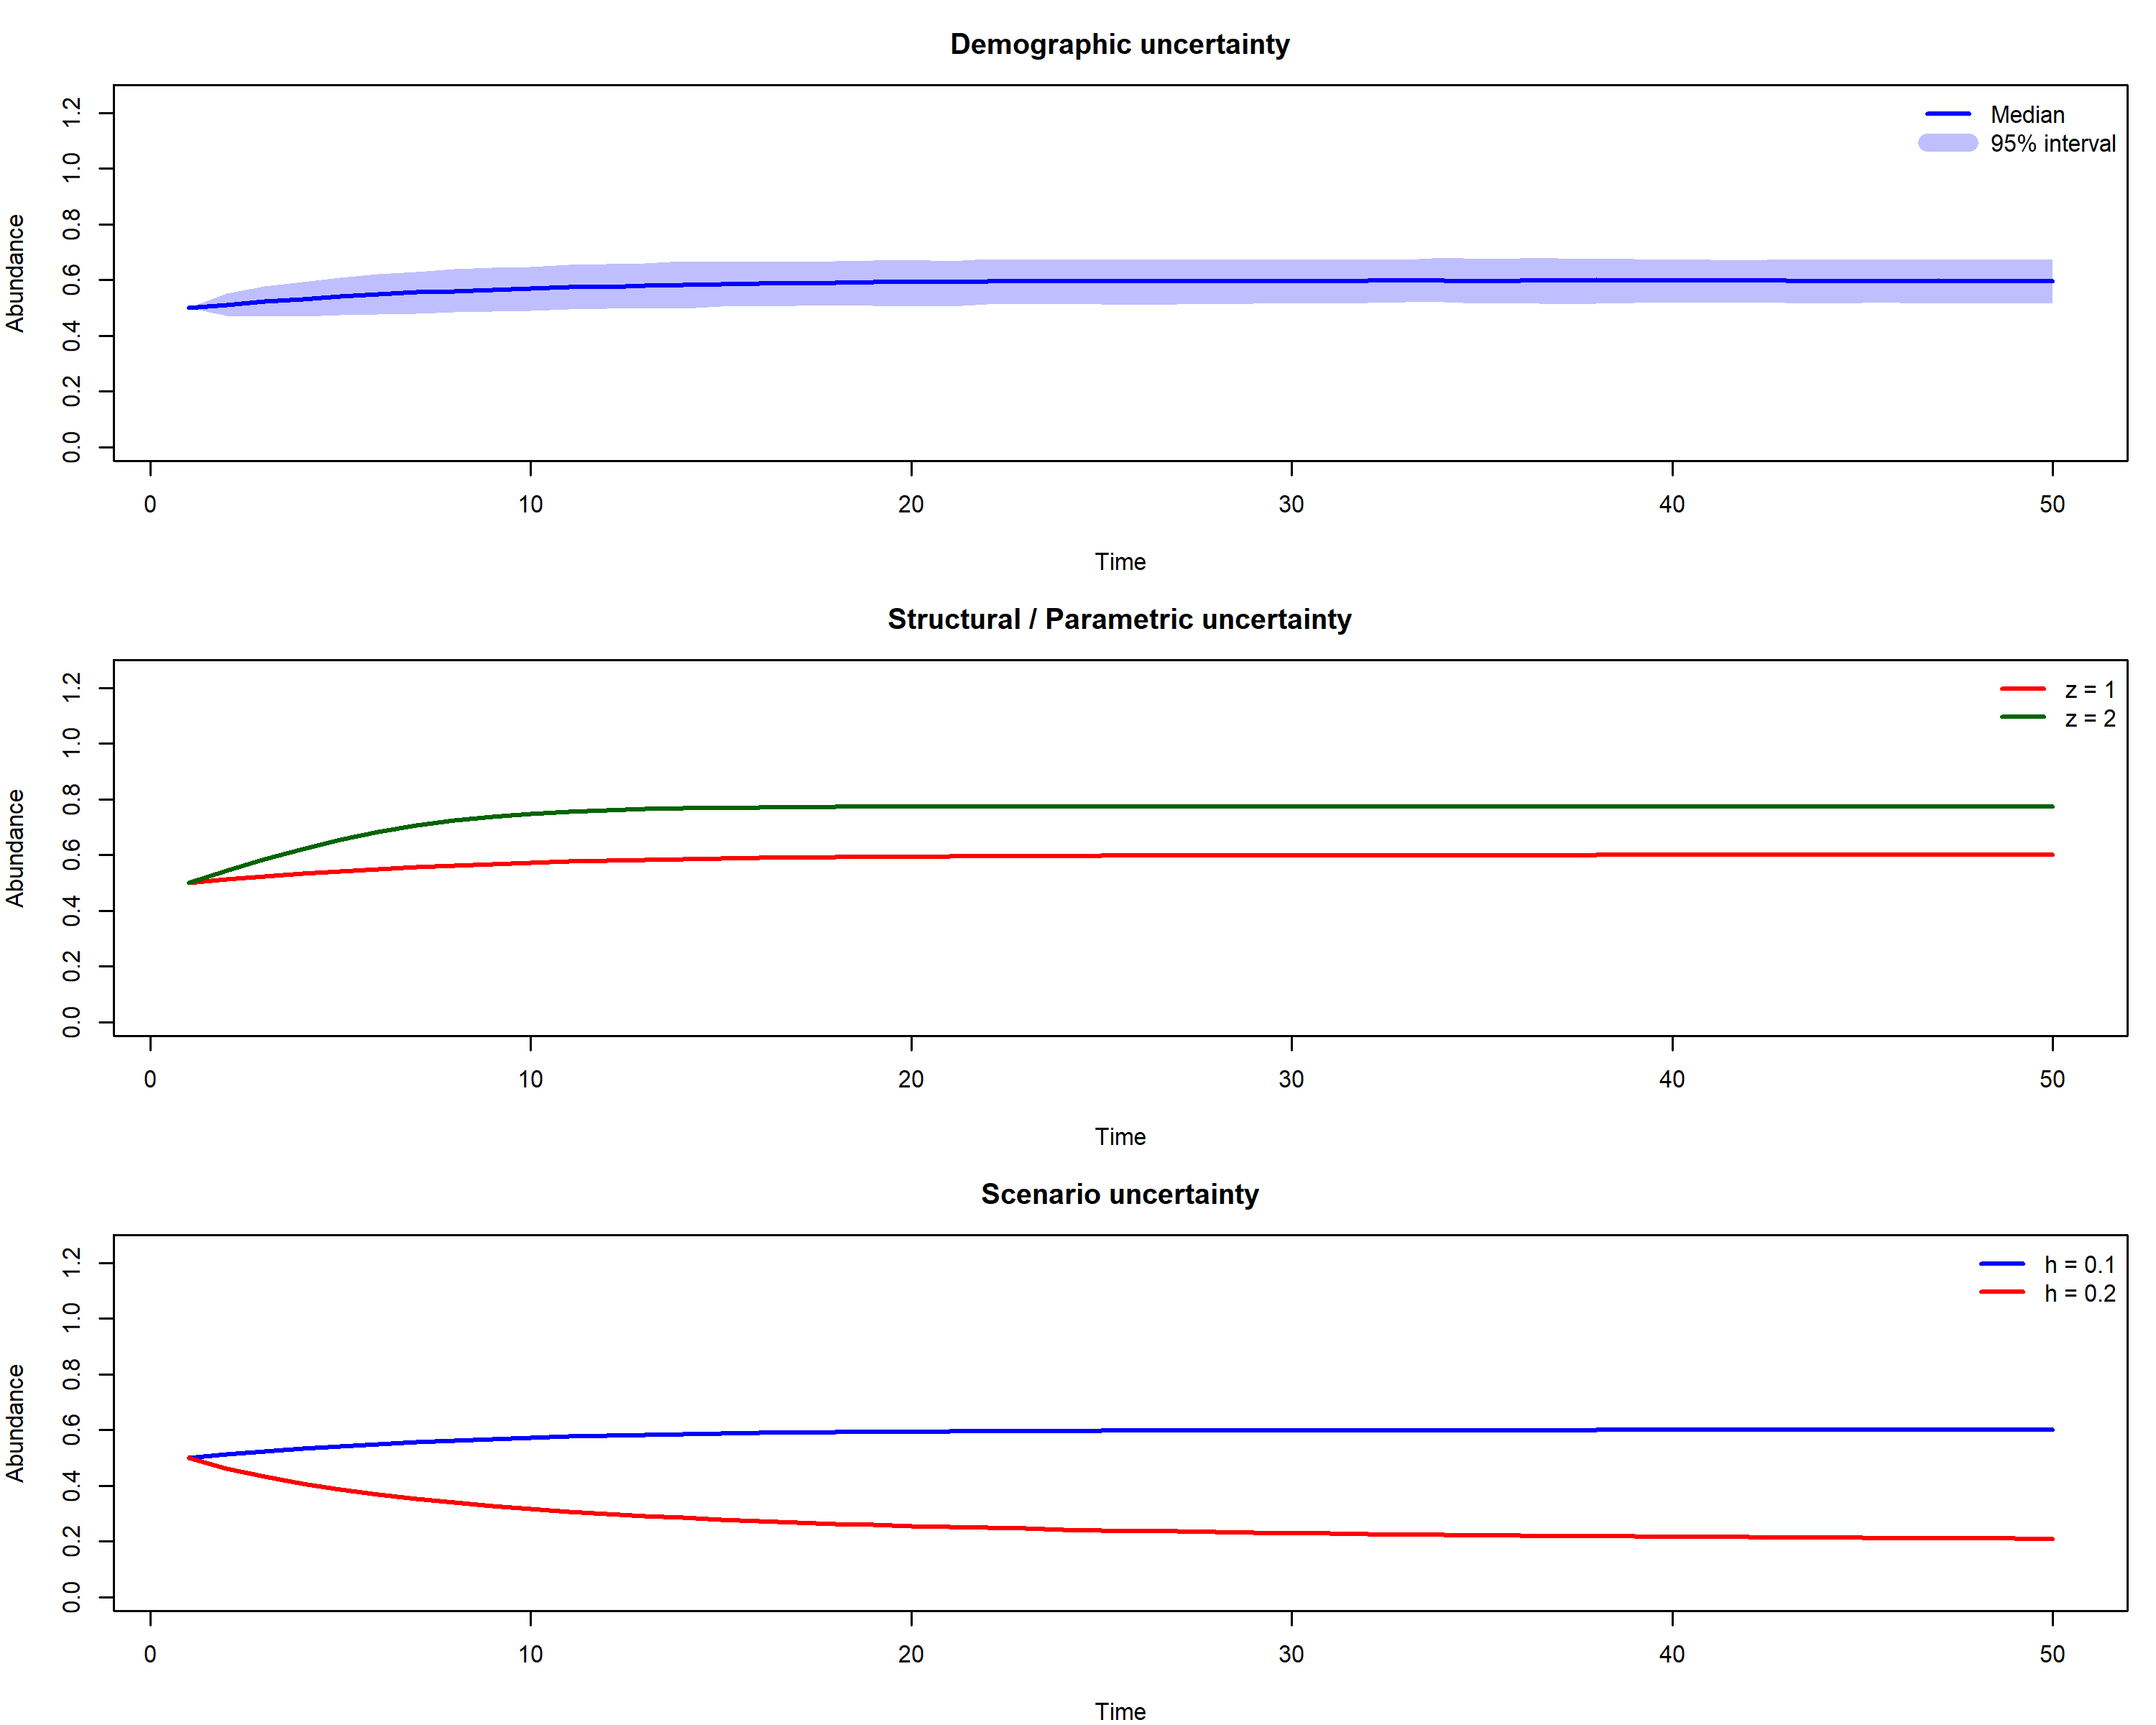
\includegraphics[width=160mm]{figures/fishery.png}
\par Original output: \texttt{week9/Fishery\_Uncertainty.tiff}. Structural uncertainty compares z = 1 and z = 2; scenario uncertainty compares h = 0.1 and h = 0.2. This document shows a lossless display conversion of the TIFF.

\clearpage\section*{Week 10 -- Vector Visualisation}
Tasks 1--3: Direct vector field visualisation, poor and improved streamlines, and line integral convolution. The complete R implementation below includes the common interpolation, integration and export functions.

{\large\bfseries\color{blue} Tasks 1--3 -- Complete R code}\par{\small Source: \texttt{week10/week10\_vectors.R}}\par
\begin{verbatim}
# Run this from the extracted project folder.
use_ggquiver <- all(vapply(c("pracma", "ggplot2", "ggquiver"),
                          requireNamespace, logical(1), quietly = TRUE))
dir.create("outputs", showWarnings = FALSE)

save_plot <- function(name, draw, width = 8, height = 7) {
  pdf(file.path("outputs", paste0(name, ".pdf")), width, height)
  draw()
  dev.off()
  if (capabilities("png")) {
    png(file.path("outputs", paste0(name, ".png")), width = width,
        height = height, units = "in", res = 180)
    draw()
    dev.off()
  }
}

# Task 1
sp <- 0.1
x_points <- seq(-2, 2, by = sp)
y_points <- seq(-1.5, 1.5, by = sp)
X <- matrix(x_points, length(y_points), length(x_points), byrow = TRUE)
Y <- matrix(y_points, length(y_points), length(x_points))
Z <- X * exp(-X^2 - Y^2)
if (use_ggquiver) {
  grad <- pracma::gradient(Z, h1 = sp, h2 = sp)
} else {
  dx <- dy <- Z * 0
  dx[, 2:(ncol(Z)-1)] <- (Z[, 3:ncol(Z)] - Z[, 1:(ncol(Z)-2)]) / (2*sp)
  dy[2:(nrow(Z)-1), ] <- (Z[3:nrow(Z), ] - Z[1:(nrow(Z)-2), ]) / (2*sp)
  dx[, 1] <- (Z[, 2] - Z[, 1]) / sp
  dx[, ncol(Z)] <- (Z[, ncol(Z)] - Z[, ncol(Z)-1]) / sp
  dy[1, ] <- (Z[2, ] - Z[1, ]) / sp
  dy[nrow(Z), ] <- (Z[nrow(Z), ] - Z[nrow(Z)-1, ]) / sp
  grad <- list(X = dx, Y = dy)
}
quiver_data <- data.frame(x = as.vector(X), y = as.vector(Y),
                          vx = as.vector(grad$X), vy = as.vector(grad$Y))
quiver_data$speed <- sqrt(quiver_data$vx^2 + quiver_data$vy^2)
if (use_ggquiver) {
  quiver_plot <- ggplot2::ggplot(quiver_data, ggplot2::aes(x, y)) +
    ggquiver::geom_quiver(ggplot2::aes(u = vx, v = vy, colour = speed)) +
    ggplot2::scale_colour_viridis_c(name = "Gradient magnitude") +
    ggplot2::coord_equal() +
    ggplot2::labs(title = "Gradient vector field", x = "x", y = "y") +
    ggplot2::theme_minimal(base_size = 12)
  save_plot("task1_quiver", function() print(quiver_plot), 9, 7)
} else {
  save_plot("task1_quiver", function() {
    par(mar = c(4, 4, 4, 1))
    plot(NA, xlim = c(-2, 2), ylim = c(-1.5, 1.5), asp = 1,
         xlab = "x", ylab = "y", main = "Gradient vector field",
         sub = "Arrow length shows gradient magnitude (scale factor 0.18)")
    with(quiver_data, {
      keep <- speed > 0.005
      arrows(x[keep], y[keep], x[keep] + 0.18*vx[keep],
             y[keep] + 0.18*vy[keep], length = 0.035, col = "#176B87")
    })
  }, 9, 7)
}

# Tasks 2 and 3 use matrix[x, y].
inside <- function(x, y, field) {
  is.finite(x) & is.finite(y) & x >= 1 & x <= nrow(field) &
    y >= 1 & y <= ncol(field)
}

sample_field <- function(field, x, y) {
  i <- pmin(floor(x), nrow(field) - 1L)
  j <- pmin(floor(y), ncol(field) - 1L)
  a <- x - i
  b <- y - j
  (1-a)*(1-b)*field[cbind(i,j)] + a*(1-b)*field[cbind(i+1,j)] +
    (1-a)*b*field[cbind(i,j+1)] + a*b*field[cbind(i+1,j+1)]
}

velocity <- function(x, y, vx, vy, normalise) {
  u <- sample_field(vx, x, y)
  v <- sample_field(vy, x, y)
  speed <- sqrt(u^2 + v^2)
  if (normalise) {
    u <- u / pmax(speed, 1e-12)
    v <- v / pmax(speed, 1e-12)
  }
  list(u = u, v = v, moving = is.finite(speed) & speed > 1e-12)
}

# Use the midpoint velocity for a smoother path.
advance <- function(x, y, vx, vy, h, normalise = FALSE) {
  nx <- ny <- rep(NA_real_, length(x))
  ids <- which(inside(x, y, vx))
  if (!length(ids)) return(list(x = nx, y = ny))
  vel <- velocity(x[ids], y[ids], vx, vy, normalise)
  mx <- x[ids] + h * vel$u / 2
  my <- y[ids] + h * vel$v / 2
  keep <- inside(mx, my, vx) & vel$moving
  ids <- ids[keep]
  if (!length(ids)) return(list(x = nx, y = ny))
  mid <- velocity(mx[keep], my[keep], vx, vy, normalise)
  tx <- x[ids] + h * mid$u
  ty <- y[ids] + h * mid$v
  keep <- inside(tx, ty, vx) & mid$moving
  nx[ids[keep]] <- tx[keep]
  ny[ids[keep]] <- ty[keep]
  list(x = nx, y = ny)
}

trace_lines <- function(seeds, vx, vy, steps, h, direction) {
  xs <- ys <- matrix(NA_real_, steps + 1L, nrow(seeds))
  xs[1, ] <- seeds$x
  ys[1, ] <- seeds$y
  for (k in seq_len(steps)) {
    pos <- advance(xs[k, ], ys[k, ], vx, vy, direction * h)
    xs[k+1, ] <- pos$x
    ys[k+1, ] <- pos$y
    if (all(is.na(pos$x))) break
  }
  list(x = xs, y = ys)
}

Vx <- readRDS("data/Vx.RDS")
Vy <- readRDS("data/Vy.RDS")
stopifnot(is.matrix(Vx), identical(dim(Vx), c(400L, 400L)),
          identical(dim(Vx), dim(Vy)), all(is.finite(Vx)), all(is.finite(Vy)))

stream_plot <- function(seeds, steps, h, title, subtitle, name) {
  forward <- trace_lines(seeds, Vx, Vy, steps, h, 1)
  backward <- trace_lines(seeds, Vx, Vy, steps, h, -1)
  visited <- matrix(FALSE, nrow(Vx), ncol(Vx))
  for (path in list(forward, backward)) {
    valid <- is.finite(path$x) & is.finite(path$y)
    visited[cbind(round(path$x[valid]), round(path$y[valid]))] <- TRUE
  }
  saveRDS(visited, file.path("outputs", paste0(name, "_visited.RDS")))
  draw <- function() {
    par(mar = c(4, 4, 4, 1))
    plot(NA, xlim = c(1, 400), ylim = c(1, 400), asp = 1,
         xlab = "x", ylab = "y", main = title, sub = subtitle)
    for (i in seq_len(nrow(seeds))) {
      lines(backward$x[, i], backward$y[, i], col = "#176B87", lwd = 0.7)
      lines(forward$x[, i], forward$y[, i], col = "#176B87", lwd = 0.7)
    }
    points(seeds$x, seeds$y, pch = 16, cex = 0.25, col = "#C45B28")
  }
  save_plot(name, draw)
}

poor_seeds <- expand.grid(x = seq(100, 300, by = 100), y = seq(100, 300, by = 100))
good_seeds <- expand.grid(x = seq(15, 385, by = 20), y = seq(15, 385, by = 20))
stream_plot(poor_seeds, 20, 0.5, "Streamlines: poor coverage",
            "9 seeds, 20 steps each way, step size 0.5", "task2_poor_streamlines")
stream_plot(good_seeds, 600, 0.5, "Streamlines: improved coverage",
            "361 seeds, 600 steps each way, step size 0.5", "task2_good_streamlines")

# Task 3
x_points <- y_points <- seq_len(400)
X <- matrix(x_points, 400, 400)
Y <- matrix(y_points, 400, 400, byrow = TRUE)
lic_vx <- X * (-Y + 200 - X)
lic_vy <- Y * (X + 200 - Y)
set.seed(362)
noise <- matrix(runif(400 * 400), 400, 400)

compute_lic <- function(vx, vy, texture, steps = 30, h = 1) {
  seeds <- expand.grid(x = seq_len(nrow(vx)), y = seq_len(ncol(vx)))
  total <- as.vector(texture)
  count <- rep(1L, nrow(seeds))
  for (direction in c(-1, 1)) {
    x <- seeds$x
    y <- seeds$y
    for (k in seq_len(steps)) {
      pos <- advance(x, y, vx, vy, direction * h, normalise = TRUE)
      x <- pos$x
      y <- pos$y
      ids <- which(is.finite(x) & is.finite(y))
      if (!length(ids)) break
      total[ids] <- total[ids] + texture[cbind(round(x[ids]), round(y[ids]))]
      count[ids] <- count[ids] + 1L
    }
  }
  matrix(total / count, nrow(vx), ncol(vx))
}

LIC <- compute_lic(lic_vx, lic_vy, noise)
stopifnot(all(is.finite(LIC)), all(LIC >= 0 & LIC <= 1))
saveRDS(LIC, "outputs/task3_lic.RDS")
limits <- quantile(LIC, c(0.01, 0.99))
lic_display <- pmin(pmax(LIC, limits[1]), limits[2])
save_plot("task3_lic", function() {
  par(mar = c(4, 4, 4, 1))
  image(x_points, y_points, lic_display, col = gray.colors(256, 0, 1),
        useRaster = TRUE, asp = 1, xlab = "x", ylab = "y",
        main = "Line integral convolution",
        sub = "30 steps each way, unit velocity, step size 1")
})
save_plot("task3_noise", function() {
  image(x_points, y_points, noise, col = gray.colors(256, 0, 1),
        useRaster = TRUE, asp = 1, xlab = "x", ylab = "y", main = "Starting white noise")
})
writeLines(capture.output(sessionInfo()), "outputs/session_info.txt")
message("Finished. Plots are saved in outputs.")
\end{verbatim}

\clearpage\section*{Task 1 -- Direct vector field}
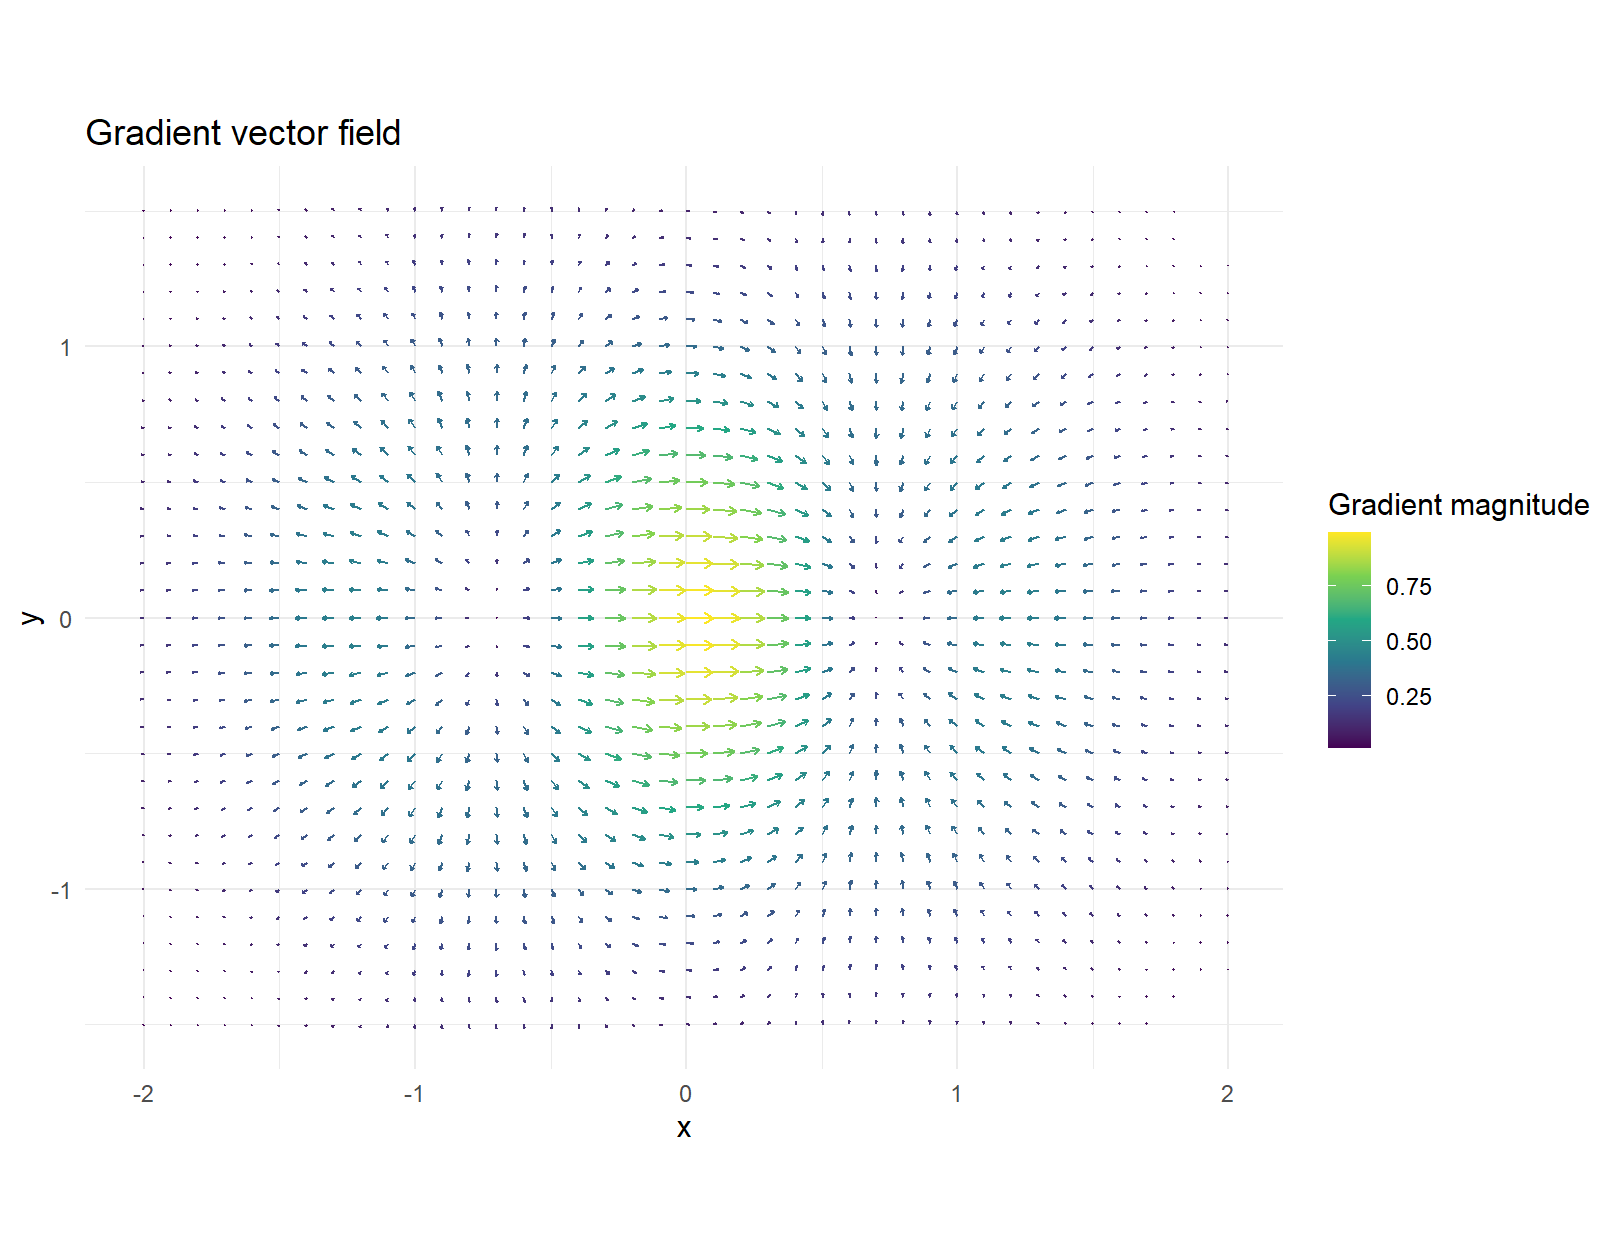
\includegraphics[width=160mm]{../week10/outputs/task1_quiver.png}
\par Quiver visualisation of the gradient of z = x exp(-x squared - y squared), sampled at grid spacing 0.1. Arrow orientation shows gradient direction and colour shows its magnitude.

\clearpage\section*{Task 2 -- Poor streamline visualisation}
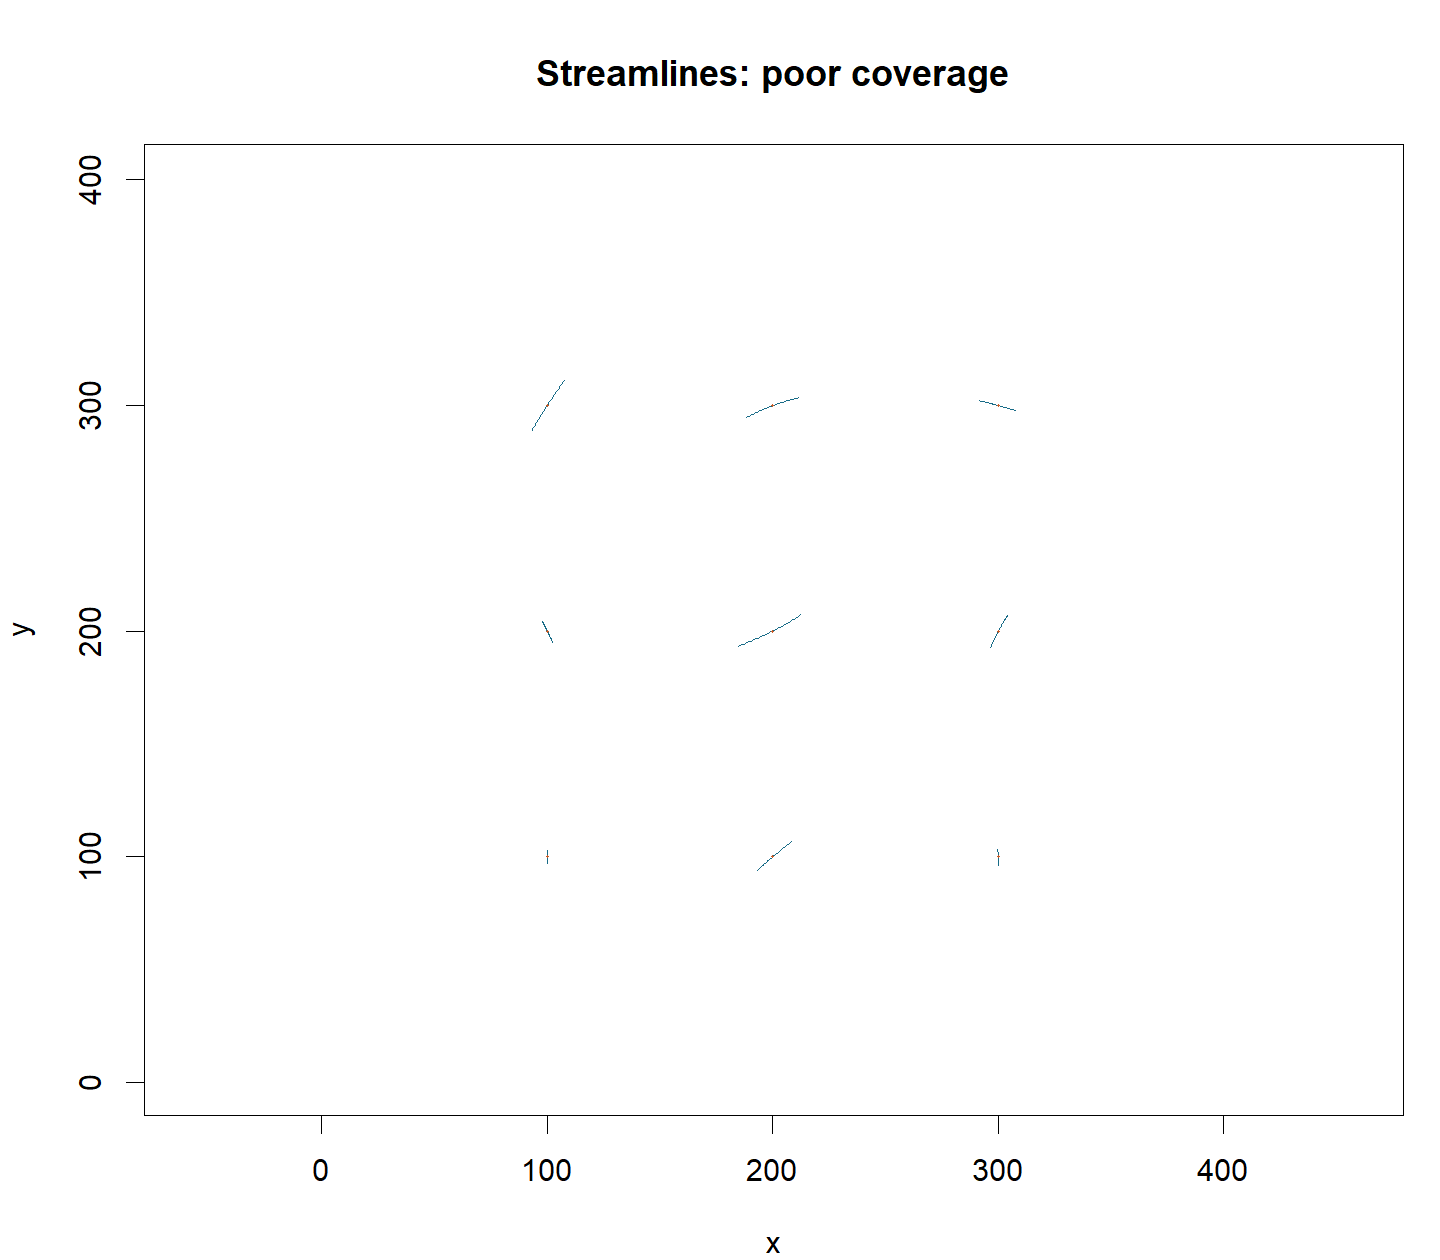
\includegraphics[width=160mm]{../week10/outputs/task2_poor_streamlines.png}
\par Nine regularly spaced seeds, 20 integration steps in each direction, step multiplier 0.5. Short paths and sparse seeds leave much of the flow structure unresolved.

\clearpage\section*{Task 2 -- Improved streamline visualisation}
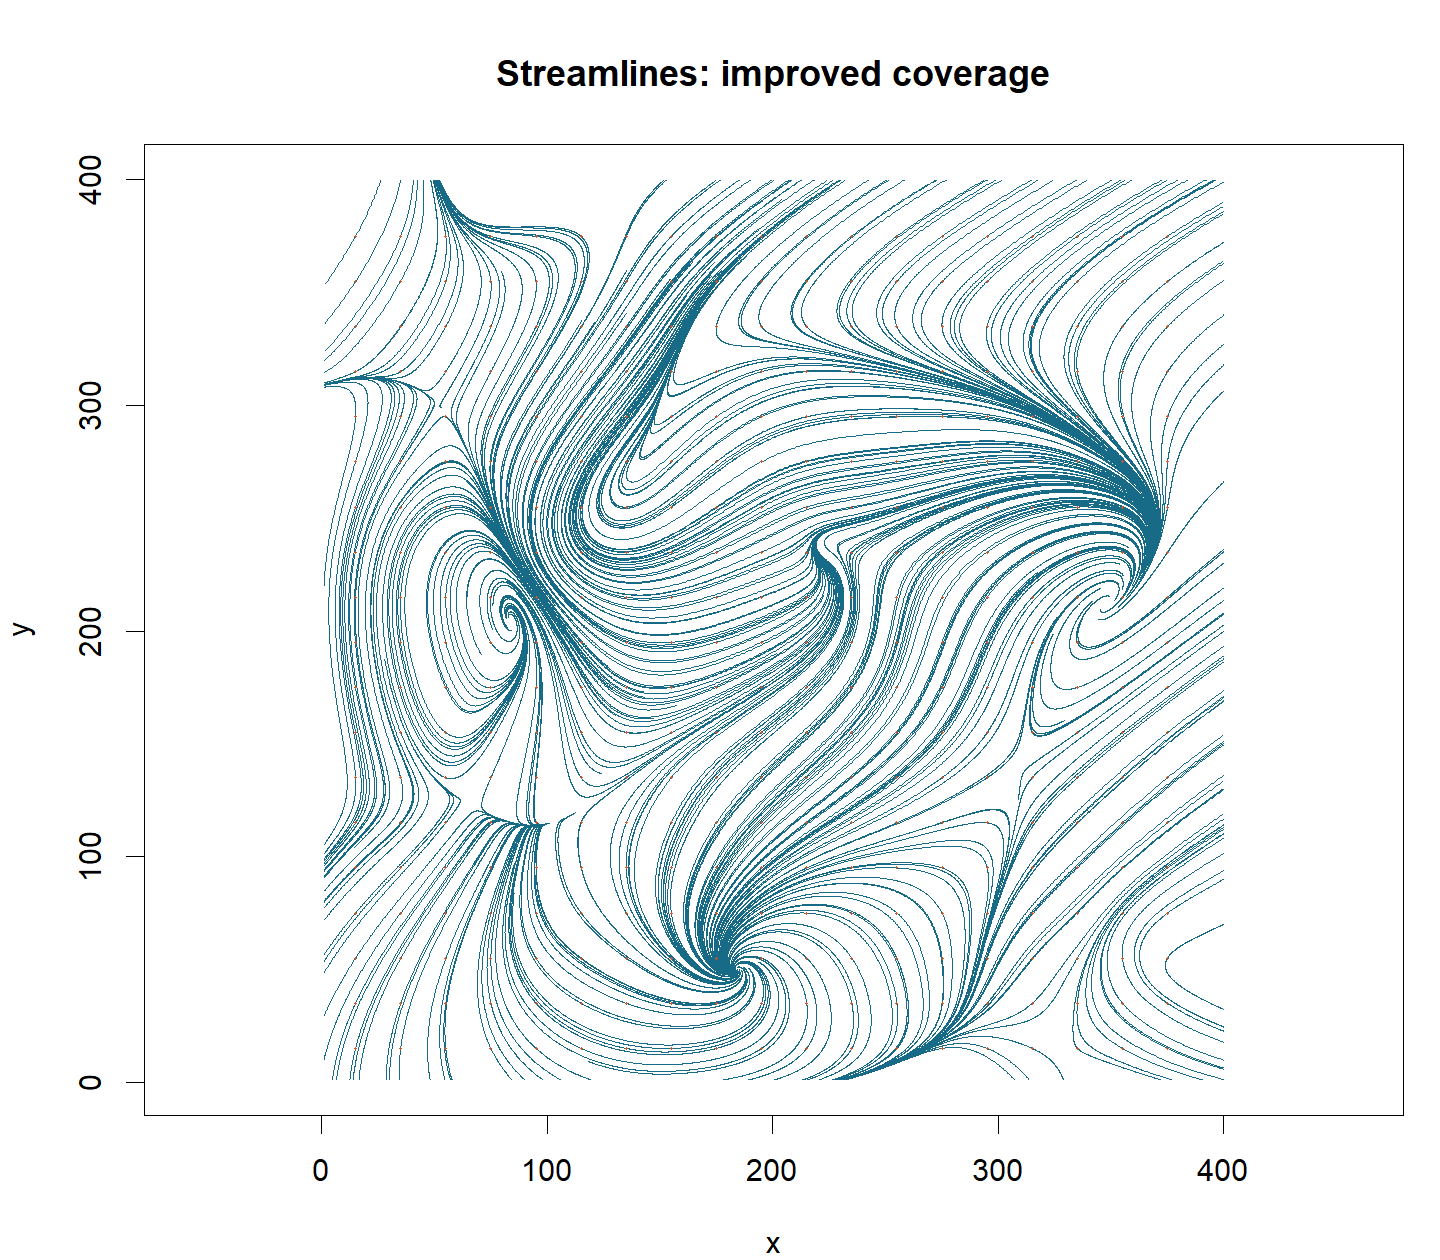
\includegraphics[width=160mm]{../week10/outputs/task2_good_streamlines.png}
\par 361 regularly spaced seeds, 600 integration steps in each direction, step multiplier 0.5. Bilinear velocity interpolation and midpoint integration improve smoothness; integration stops at the domain boundary. Orange points mark seeds.

\clearpage\section*{Task 3 -- Line integral convolution}
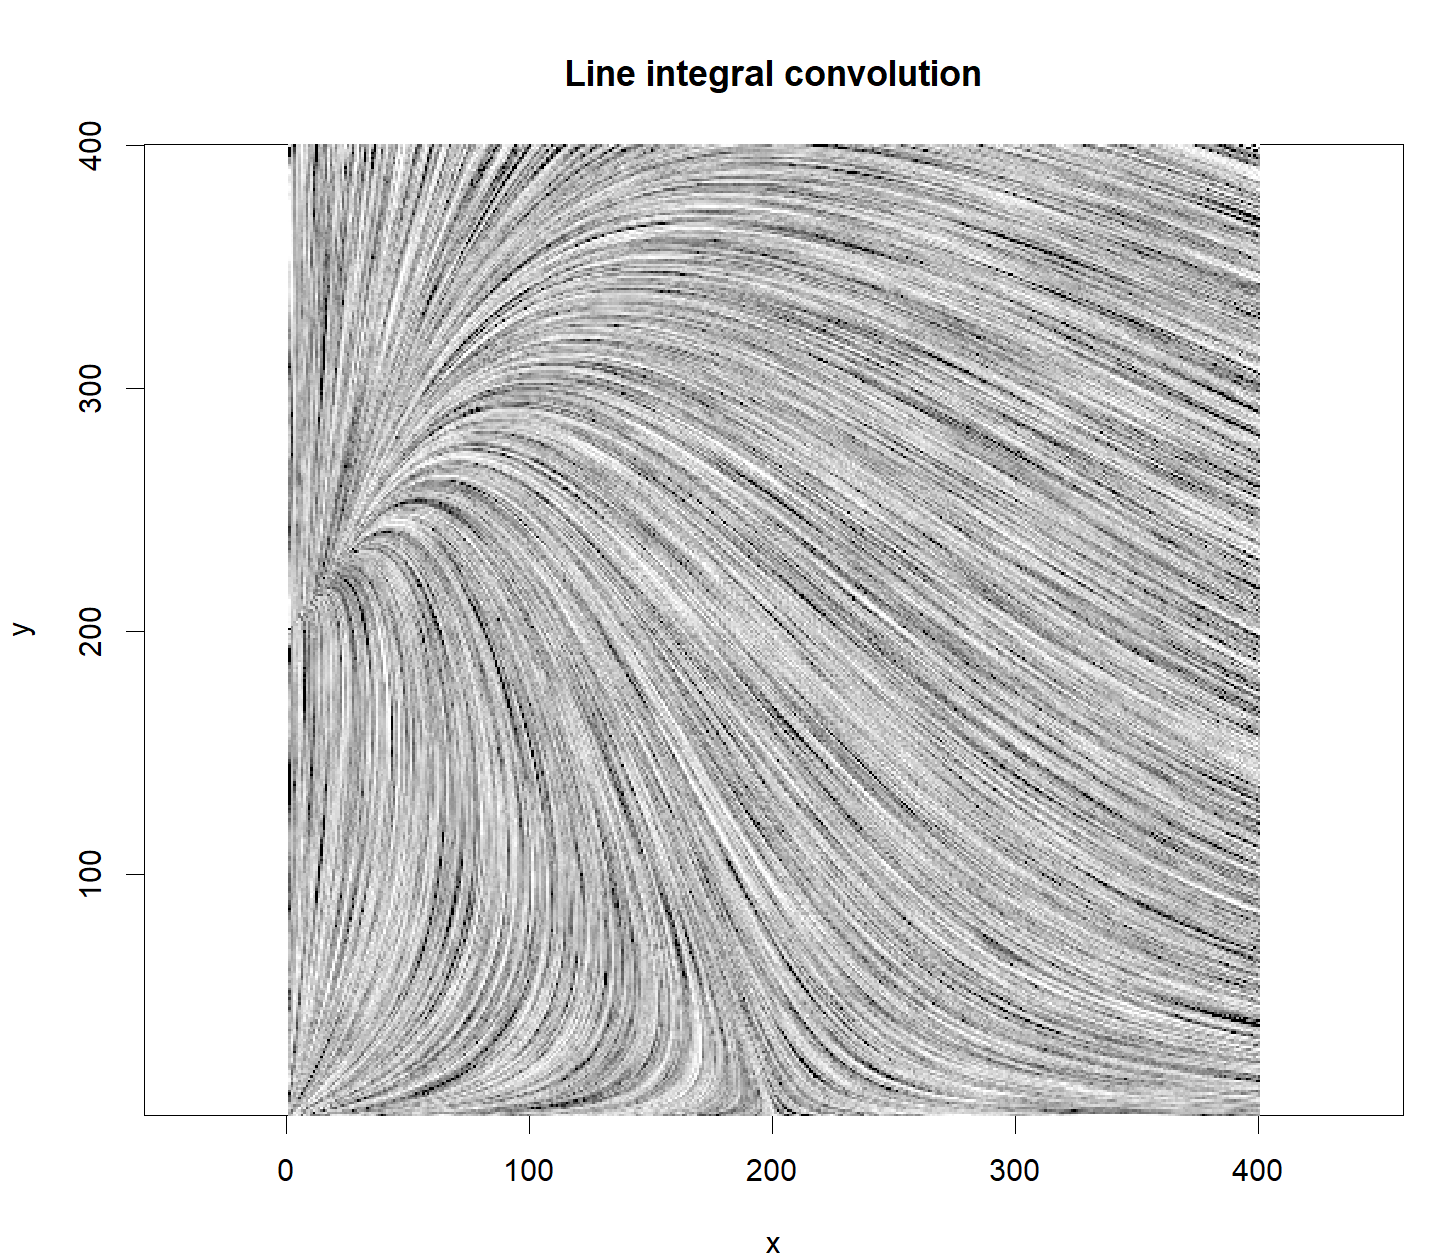
\includegraphics[width=160mm]{../week10/outputs/task3_lic.png}
\par Every grid point is a seed. Integration uses up to 30 steps each way at unit step size. Both optional extensions are implemented: normalised velocity and division by the actual sample count near boundaries. Display contrast is clipped at the 1st and 99th percentiles; the original LIC values are saved separately.

\clearpage\section*{Task 3 -- Additional starting texture}
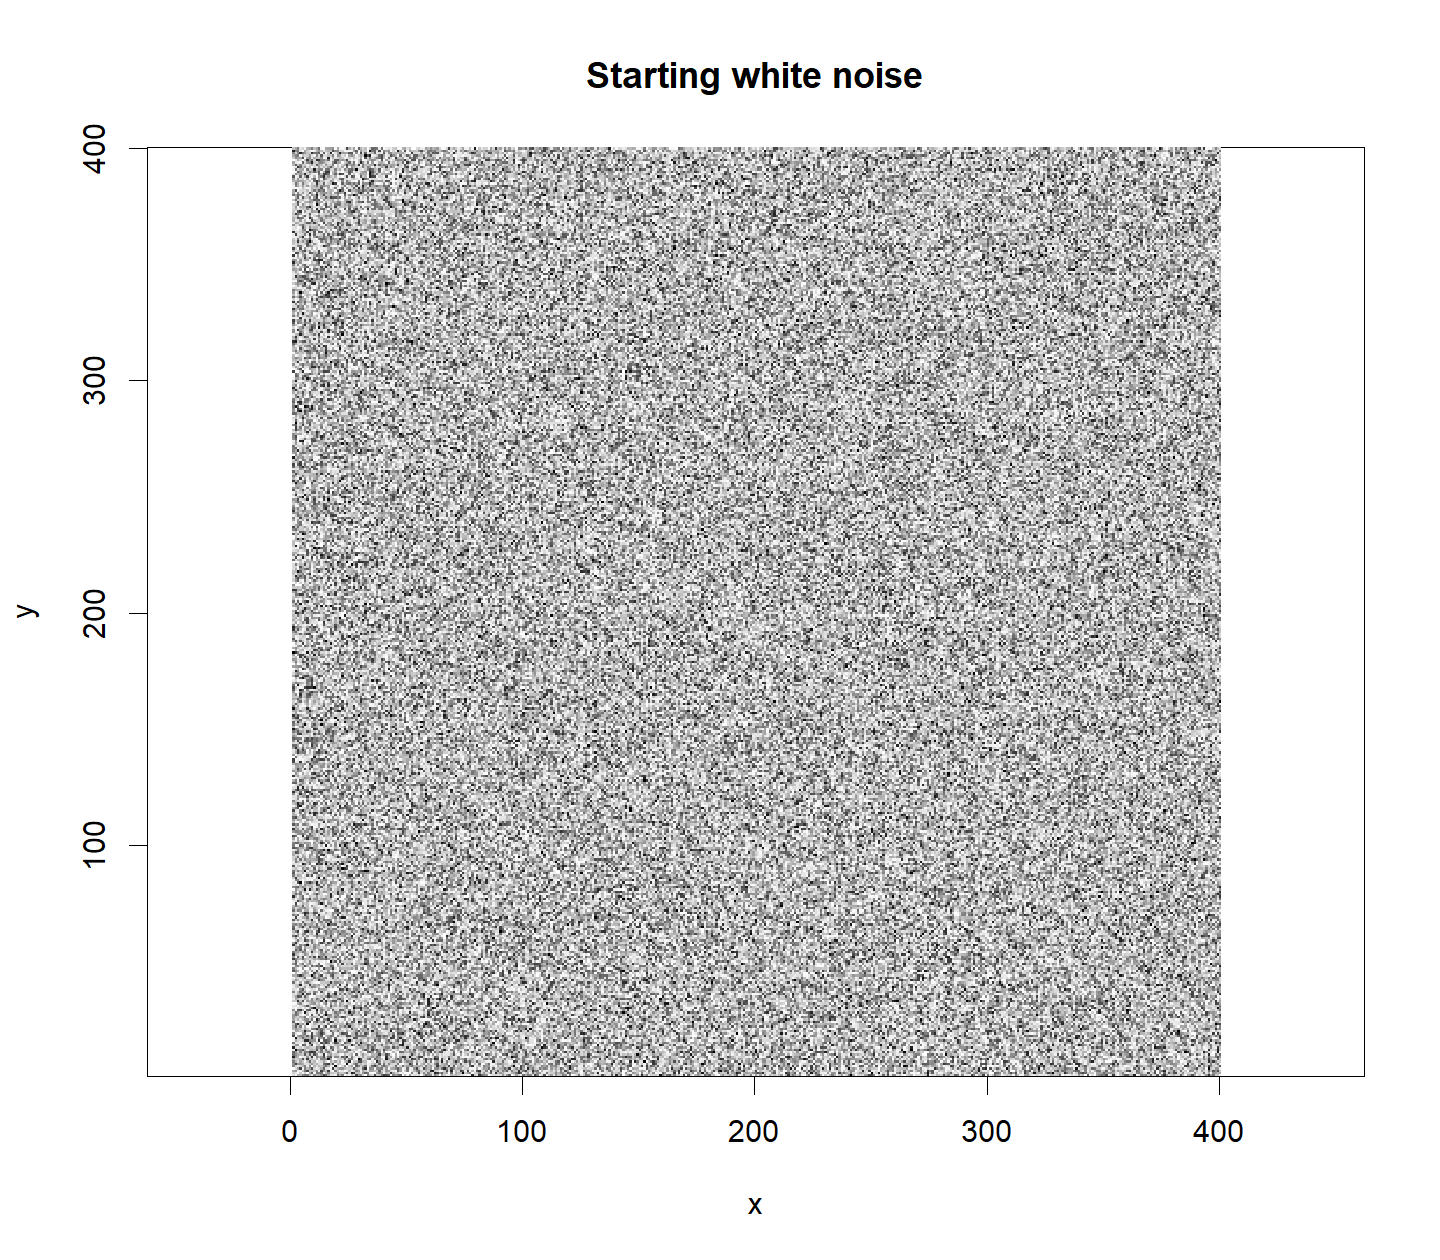
\includegraphics[width=160mm]{../week10/outputs/task3_noise.png}
\par Starting white noise generated with seed 362, before convolution along the vector field.

\clearpage\section*{Week 11 -- Visualising High Dimensional Data}
Tasks 1--4: Iris scatter plot matrix, covariance-based PCA, and LDA projection and species separation. The complete submission code generates the plots and numerical results shown below.

The LDA examples in slides 6--7 use columns 1 and 3 (sepal length and petal length), while the final task slide asks for the first two dimensions. Both variable selections are supplied. The projection search evaluates unit vectors over 1,000 angles from 0 to pi, using between-class covariance divided by total covariance.
{\large\bfseries\color{blue} Tasks 1--4 -- R code}\par{\small Source: \texttt{submission/code/week11\_corrected.R (run from week11)}}\par
\begin{verbatim}
# Run from 3.2/week11. Original pract1.R remains unchanged.
library(paletteer)
library(ggplot2)
colors <- paletteer_d("ochRe::lorikeet", n = 3)
data(iris)
speciesID <- as.numeric(iris$Species)
out <- "../submission/figures"
start_plot <- function(name) {
  png(file.path(out, paste0(name, ".png")), width=1800, height=1350, res=180)
}
# Task 1: each distinct numerical pair, coloured and marked by species.
start_plot("week11_pairs")
pairs(iris[,1:4], col=colors[speciesID], pch=speciesID, lower.panel=NULL)
par(xpd=NA)
legend("bottomleft", col=colors, pch=1:3, legend=levels(iris$Species))
dev.off()
# Task 2: mean-centred covariance PCA, matching the practical.
X <- scale(as.matrix(iris[,1:4]), center=TRUE, scale=FALSE)
Eigen <- eigen(cov(X))
Z <- X %*% Eigen$vectors[,1:2]
start_plot("week11_pca")
plot(Z, col=colors[speciesID], pch=speciesID,
     xlab="Principal Component 1", ylab="Principal Component 2", main="PCA of Iris Data")
legend("topright", col=colors, pch=1:3, legend=levels(iris$Species))
dev.off()
# Tasks 3-4: search unit vectors to maximise Fisher's criterion.
\end{verbatim}

\clearpage{\Large\bfseries\color{navy} Week 11 -- LDA code}\par
\begin{verbatim}
# Slides 6-7 request columns 1 and 3; final task slide says first two.
# Supply both interpretations explicitly.
results <- character()
for (cols in list(c(1,3), c(1,2))) {
  X <- scale(as.matrix(iris[,cols]))
  Sigma <- cov(X)
  Sigma_b <- matrix(0,2,2)
  for (k in 1:3) {
    delta <- colMeans(X[speciesID==k,]) - colMeans(X)
    Sigma_b <- Sigma_b + tcrossprod(delta)/3
  }
  fisher <- function(w) as.numeric(t(w)%*%Sigma_b%*%w / (t(w)%*%Sigma%*%w))
  angles <- seq(0,pi,length.out=1000)
  J <- vapply(angles, function(a) fisher(c(cos(a),sin(a))), numeric(1))
  best <- which.max(J)
  W <- c(cos(angles[best]),sin(angles[best]))
  W <- W/sqrt(sum(W^2))
  Y <- as.vector(X%*%W)
  tag <- if (cols[2]==3) "main" else "first_two"
  results <- c(results, paste("Variables:",paste(colnames(X),collapse=", ")),
               sprintf("W = [%.8f; %.8f]",W[1],W[2]), sprintf("J(W) = %.8f",fisher(W)), "")
  start_plot(paste0("week11_lda_direction_",tag))
  plot(X, col=colors[speciesID], pch=speciesID,
       xlab=paste("Standardised",colnames(X)[1]),
       ylab=paste("Standardised",colnames(X)[2]), main="LDA Projection Direction")
  lines(c(-2*W[1],2*W[1]),c(-2*W[2],2*W[2]),lwd=2)
  legend("topright",col=colors,pch=1:3,legend=levels(iris$Species))
  dev.off()
  start_plot(paste0("week11_lda_histogram_",tag))
  d <- data.frame(Projection=Y,Species=iris$Species)
  print(ggplot(d,aes(Projection,fill=Species))+
    geom_histogram(colour="grey50",alpha=0.4,position="identity",bins=20)+
    scale_fill_manual(values=colors)+
    labs(title=paste("LDA:",paste(colnames(X),collapse=" and ")),
         x="Projection onto W",y="Count"))
  dev.off()
}
writeLines(results,file.path(out,"week11_lda_results.txt"))
print(results)
\end{verbatim}

\clearpage\section*{Task 1 -- Iris scatter plot matrix}
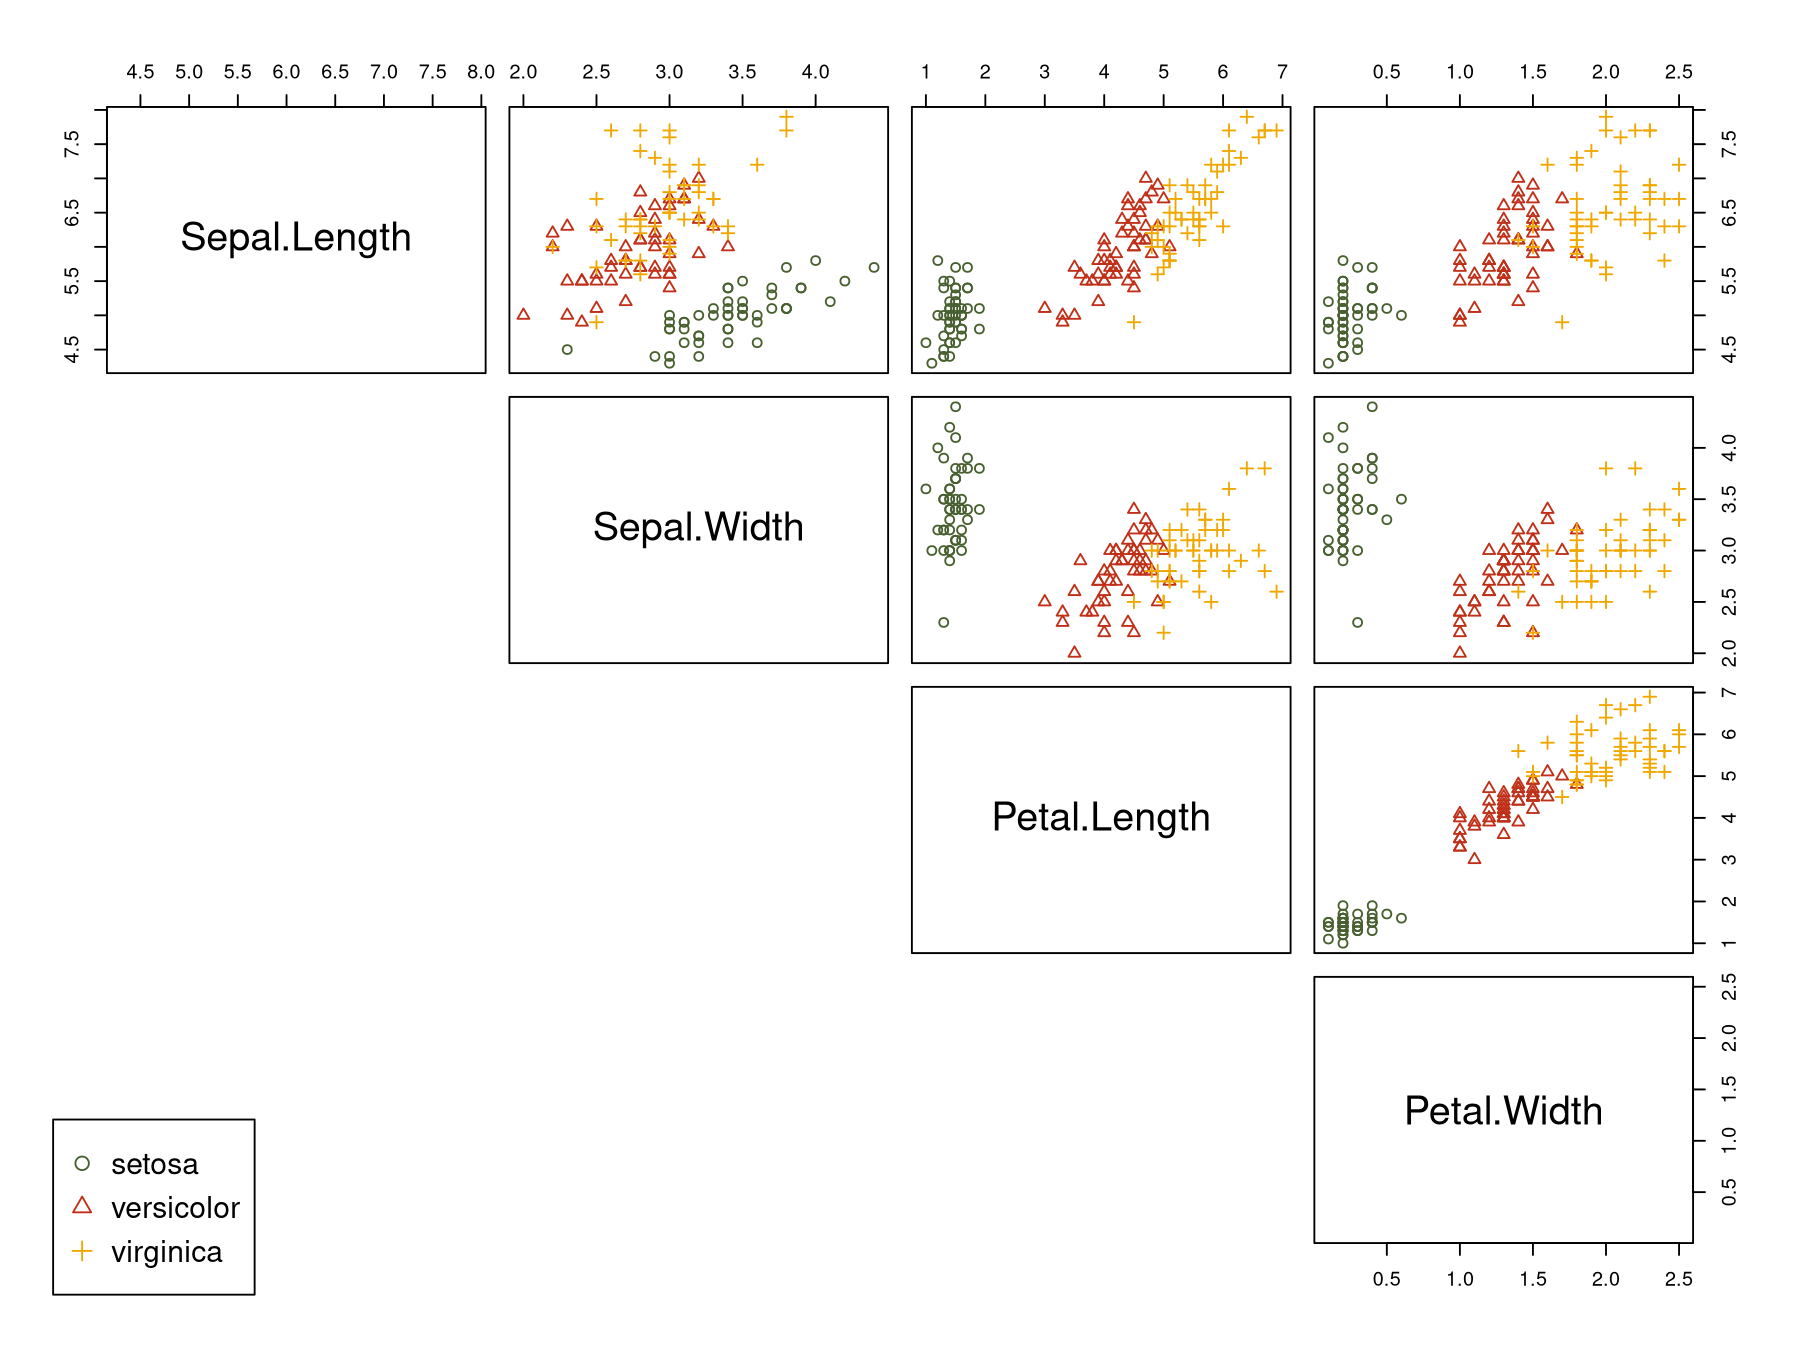
\includegraphics[width=160mm]{figures/week11_pairs.png}
\par All six distinct pairs of the four numerical iris variables are displayed. Species are distinguished by both colour and symbol; duplicate lower-triangle panels are omitted.

\clearpage\section*{Task 2 -- Principal component projection}
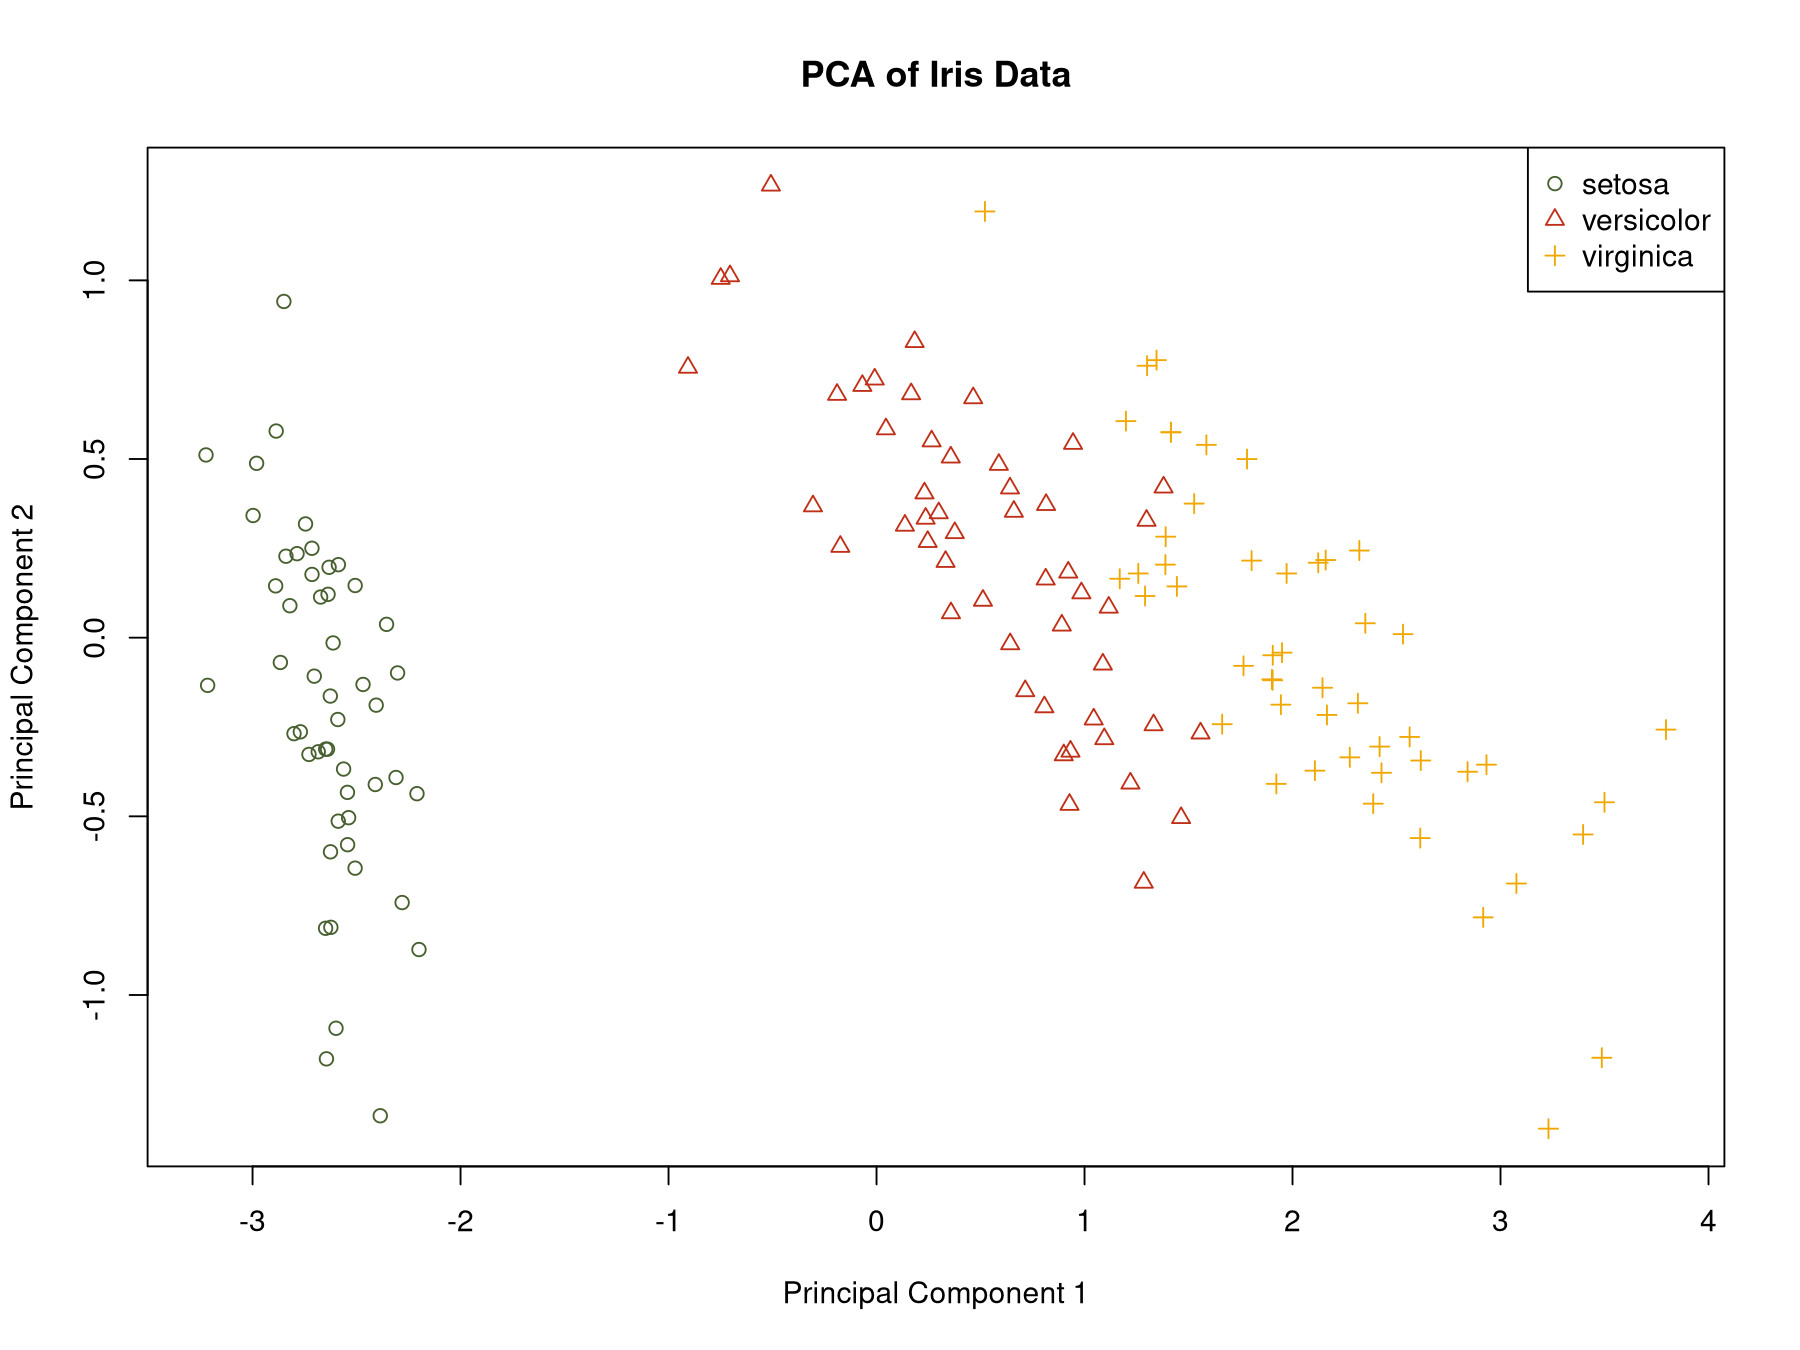
\includegraphics[width=160mm]{figures/week11_pca.png}
\par The mean-centred four-variable iris data are projected onto the two eigenvectors of the covariance matrix with the largest eigenvalues, with species indicated by colour and symbol.

\clearpage\section*{Task 3 -- LDA projection results}
The reported vectors have unit length. J(W) is the Fisher criterion implemented in the code. Reversing both signs of W gives the same separation and criterion value.

\begin{verbatim}
Variables: Sepal.Length, Petal.Length
W = [-0.21989222; 0.97552417]
J(W) = 0.95251145

Variables: Sepal.Length, Sepal.Width
W = [-0.82674458; 0.56257746]
J(W) = 0.80126605

\end{verbatim}
The first result follows the worked LDA instructions (columns 1 and 3). The second follows the final task wording literally (columns 1 and 2). Each corresponding species histogram follows.
\clearpage\section*{Task 4 -- LDA projection direction}
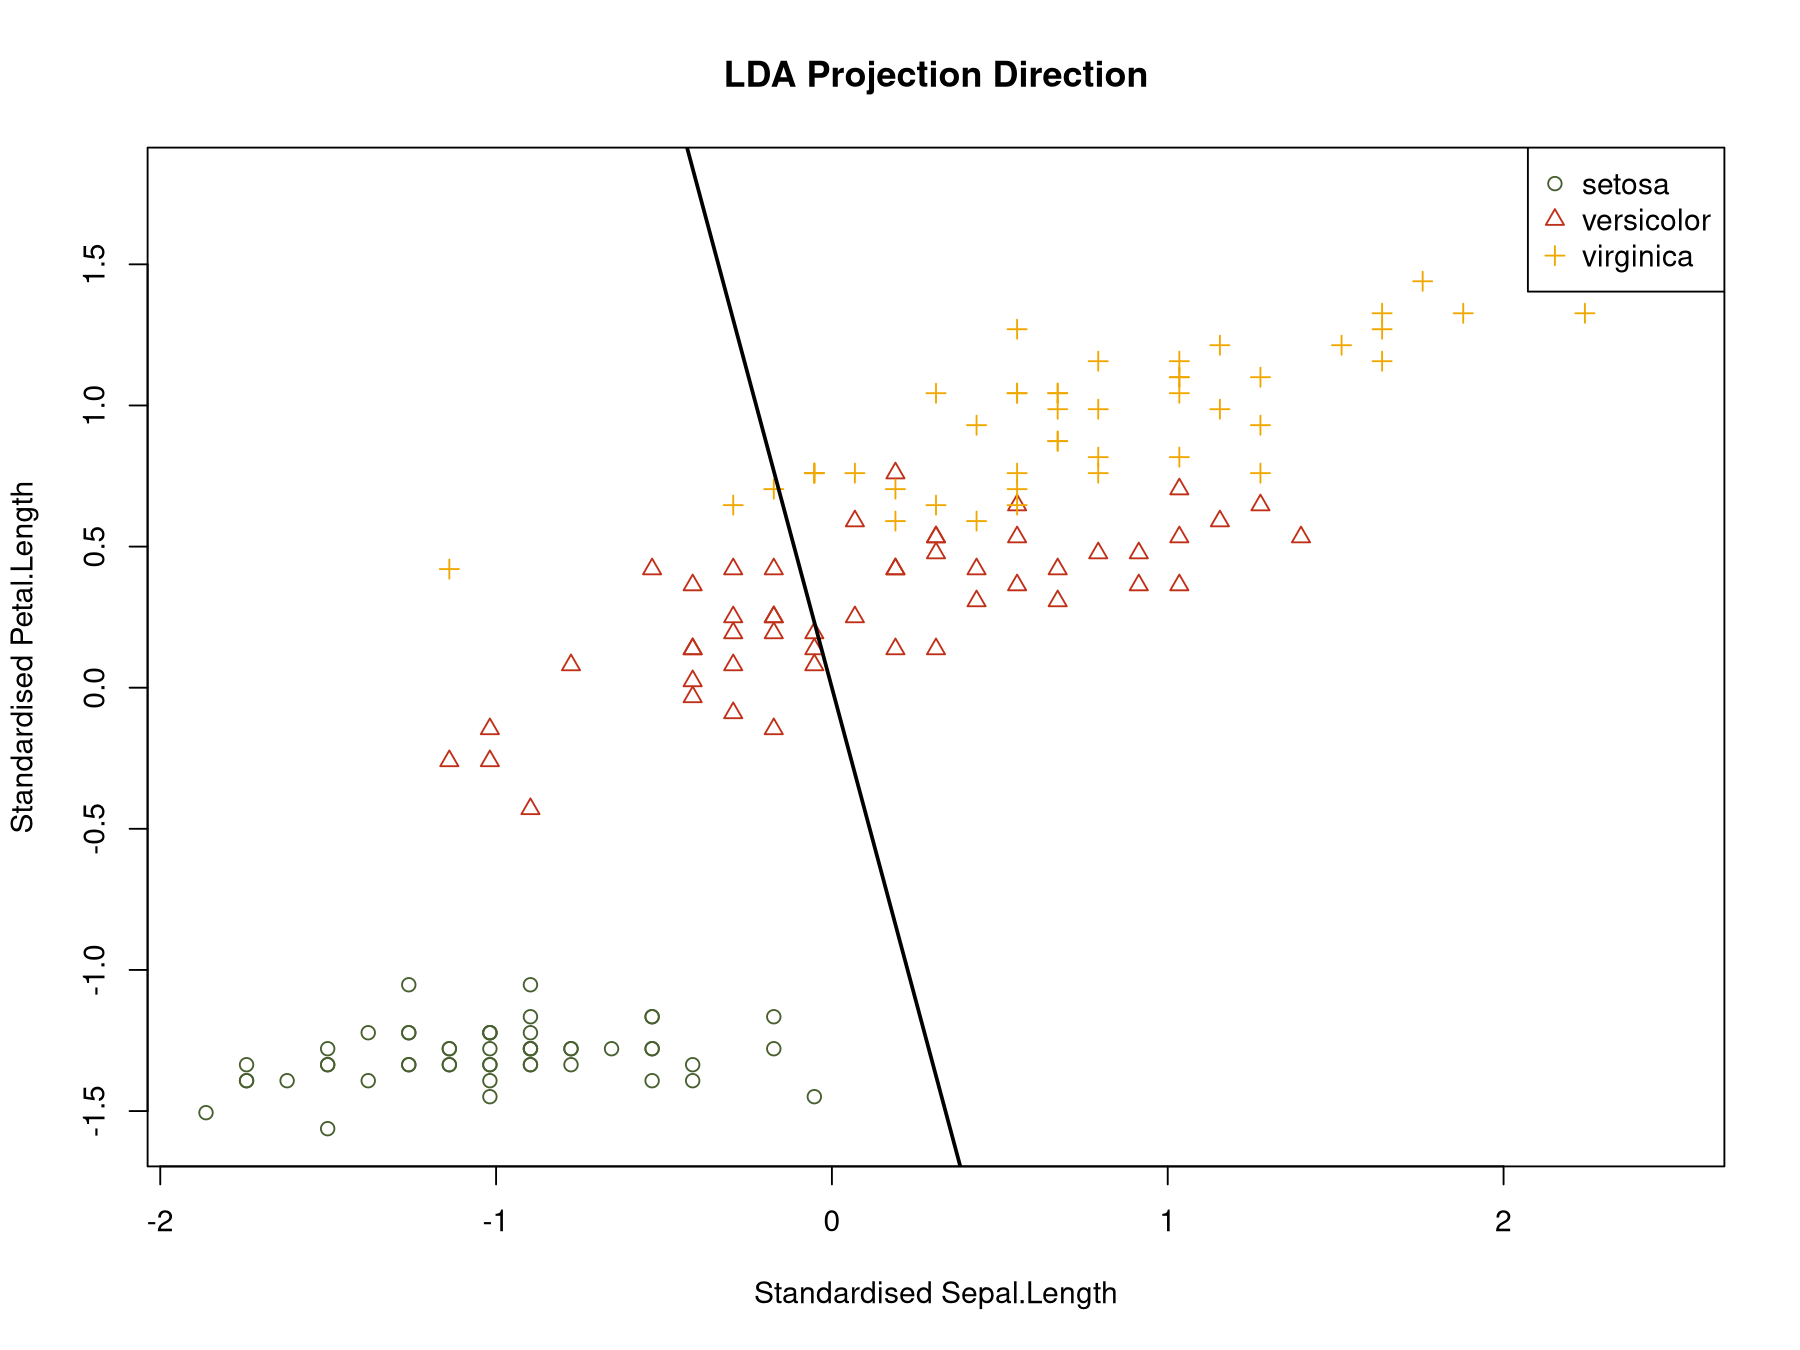
\includegraphics[width=160mm]{figures/week11_lda_direction_main.png}
\par Standardised sepal length and petal length, following slides 6--7. The black line gives the optimised projection direction.

\clearpage\section*{Task 4 -- Species separation along W}
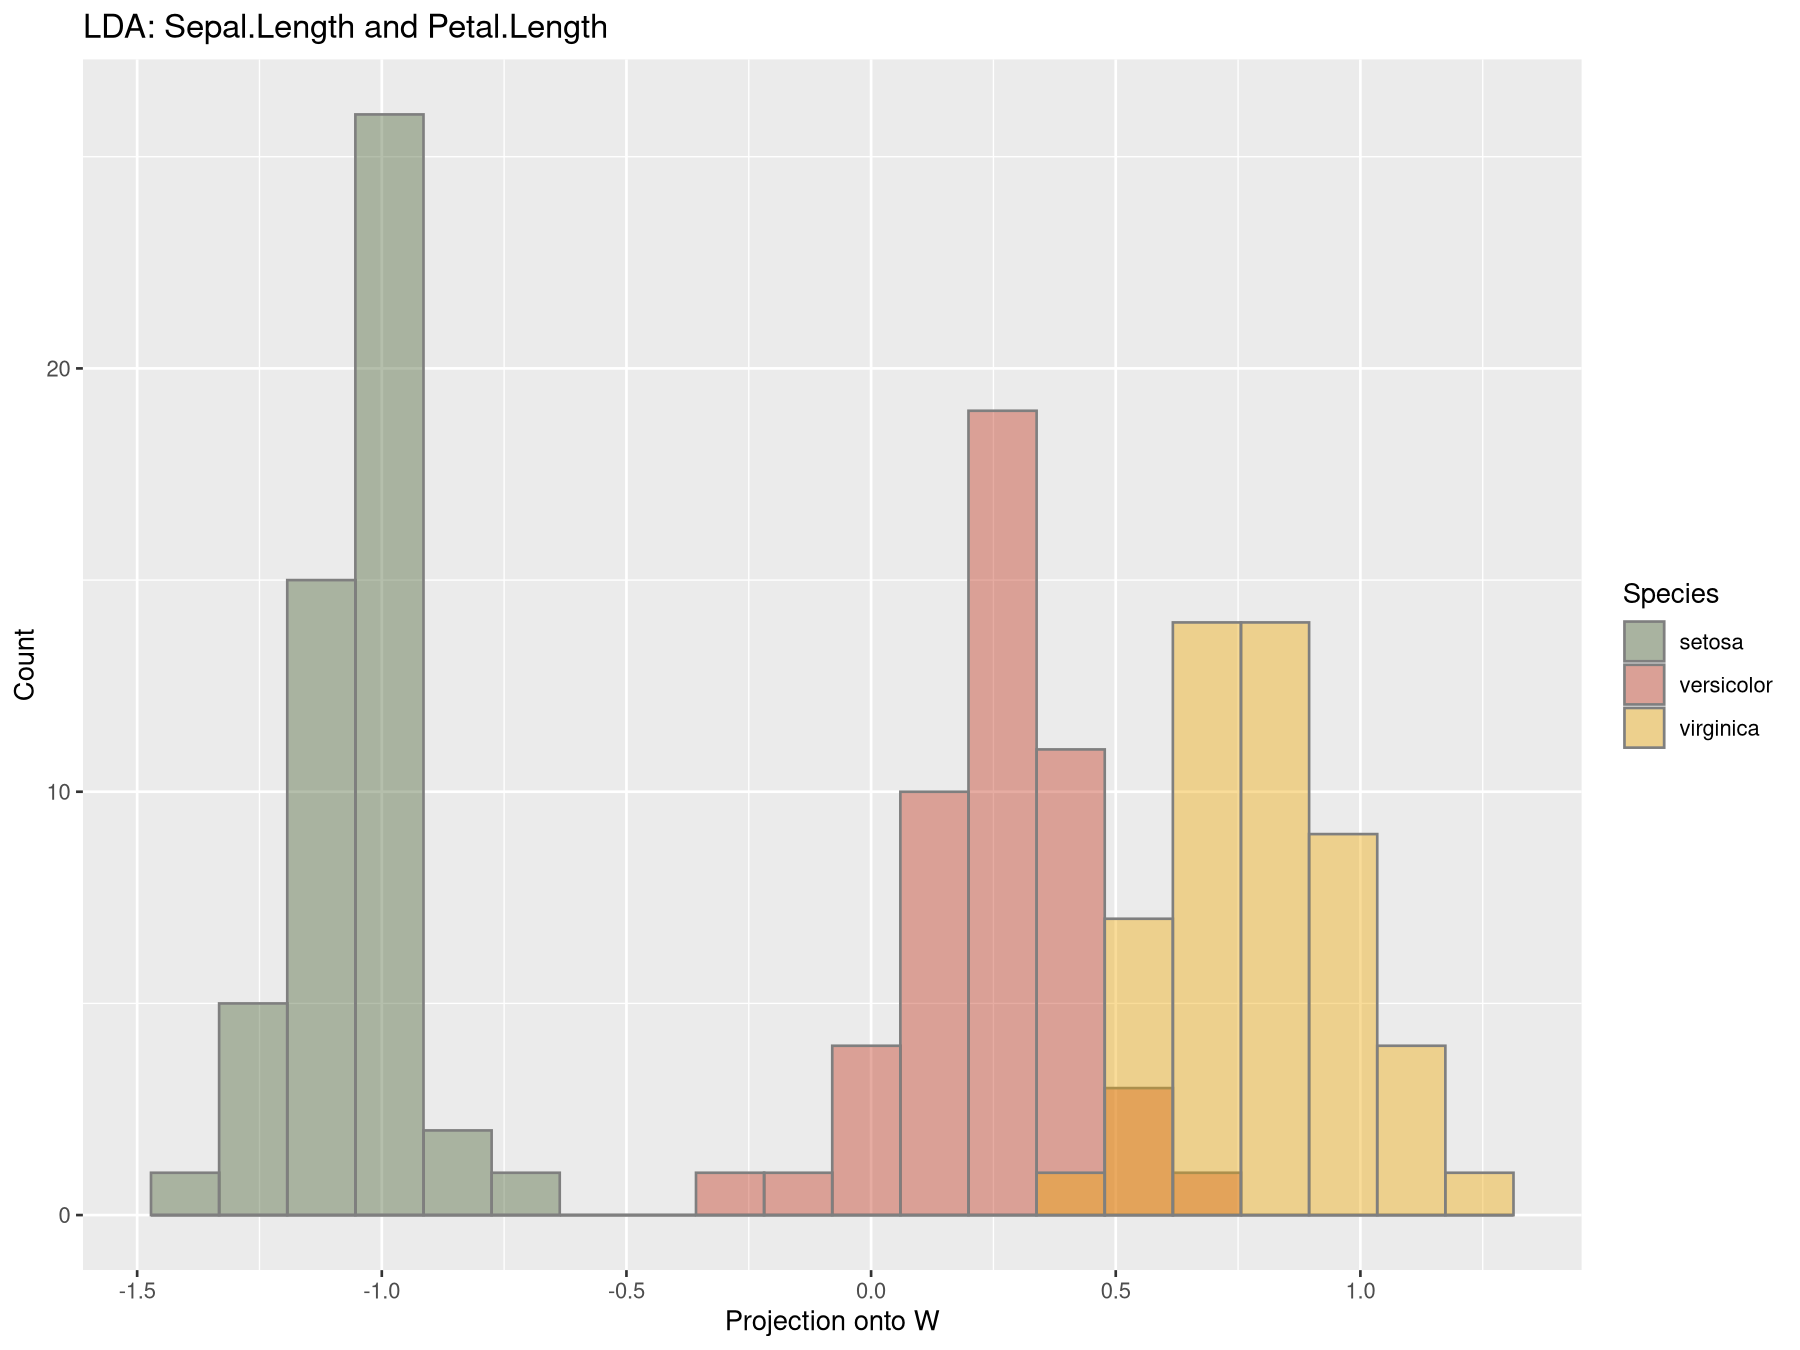
\includegraphics[width=160mm]{figures/week11_lda_histogram_main.png}
\par Histogram of projections onto the optimised vector for sepal length and petal length. Setosa separates clearly; versicolor and virginica overlap.

\clearpage\section*{Tasks 3--4 -- First two dimensions}
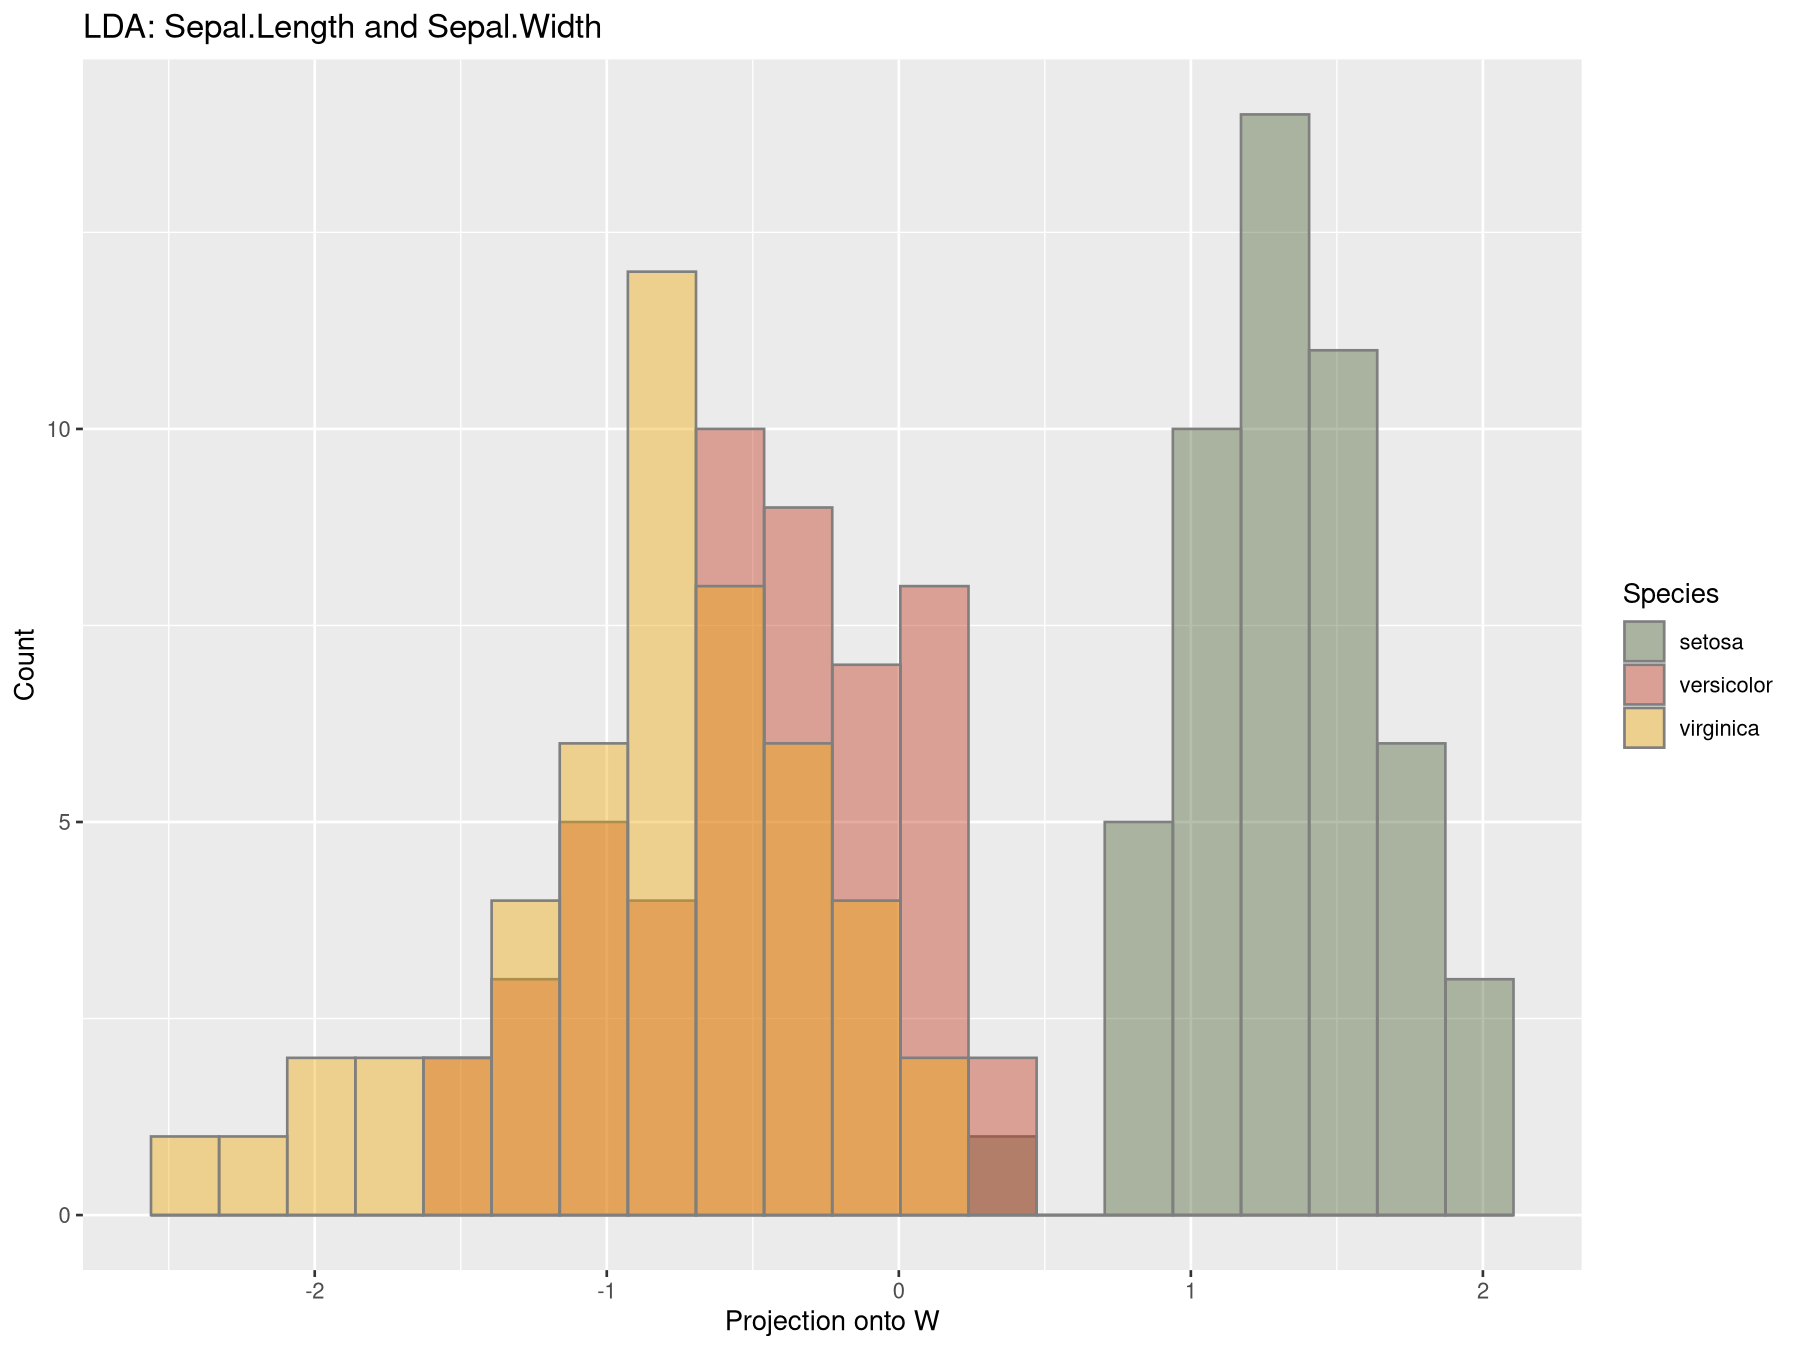
\includegraphics[width=160mm]{figures/week11_lda_histogram_first_two.png}
\par Supplementary histogram for sepal length and sepal width, covering the final task slide wording. The matching W and J(W) are reported above.

\end{document}